% ******************************* PhD Thesis Template **************************
% Please have a look at the README.md file for info on how to use the template

\documentclass[a4paper,12pt,times,numbered,print,index]{Classes/PhDThesisPSnPDF}

% ******************************************************************************
% ******************************* Class Options ********************************
% *********************** See README for more details **************************
% ******************************************************************************

% `a4paper'(The University of Cambridge PhD thesis guidelines recommends a page
% size a4 - default option) or `a5paper': A5 Paper size is also allowed as per
% the Cambridge University Engineering Deparment guidelines for PhD thesis
%
% `11pt' or `12pt'(default): Font Size 10pt is NOT recommended by the University
% guidelines
%
% `oneside' or `twoside'(default): Printing double side (twoside) or single
% side.
%
% `print': Use `print' for print version with appropriate margins and page
% layout. Leaving the options field blank will activate Online version.
%
% `index': For index at the end of the thesis
%
% `draftclassic': For draft mode without loading any images (same as draft in book)
%
% `draft': Special draft mode with line numbers, images, and water mark with
% timestamp and custom text. Position of the text can also be modified.
%
% `abstract': To generate only the title page and abstract page with
% dissertation title and name, to submit to the Student Registry
%
% `chapter`: This option enables only the specified chapter and it's references
%  Useful for review and corrections.
%
% ************************* Custom Page Margins ********************************
%
% `custommargin`: Use `custommargin' in options to activate custom page margins,
% which can be defined in the preamble.tex. Custom margin will override
% print/online margin setup.
%
% *********************** Choosing the Fonts in Class Options ******************
%
% `times' : Times font with math support. (The Cambridge University guidelines
% recommend using times)
%
% `fourier': Utopia Font with Fourier Math font (Font has to be installed)
%            It's a free font.
%
% `customfont': Use `customfont' option in the document class and load the
% package in the preamble.tex
%
% default or leave empty: `Latin Modern' font will be loaded.
%
% ********************** Choosing the Bibliography style ***********************
%
% `authoryear': For author-year citation eg., Krishna (2013)
%
% `numbered': (Default Option) For numbered and sorted citation e.g., [1,5,2]
%
% `custombib': Define your own bibliography style in the `preamble.tex' file.
%              `\RequirePackage[square, sort, numbers, authoryear]{natbib}'.
%              This can be also used to load biblatex instead of natbib
%              (See Preamble)
%
% **************************** Choosing the Page Style *************************
%
% `default (leave empty)': For Page Numbers in Header (Left Even, Right Odd) and
% Chapter Name in Header (Right Even) and Section Name (Left Odd). Blank Footer.
%
% `PageStyleI': Chapter Name next & Page Number on Even Side (Left Even).
% Section Name & Page Number in Header on Odd Side (Right Odd). Footer is empty.
%
% `PageStyleII': Chapter Name on Even Side (Left Even) in Header. Section Number
% and Section Name in Header on Odd Side (Right Odd). Page numbering in footer

% Uncomment to change page style
%\pagestyle{PageStyleII}

% ********************************** Preamble **********************************
% Preamble: Contains packages and user-defined commands and settings
% ******************************************************************************
% ****************************** Custom Margin *********************************

% Add `custommargin' in the document class options to use this section
% Set {innerside margin / outerside margin / topmargin / bottom margin}  and
% other page dimensions
\ifsetCustomMargin
  \RequirePackage[left=37mm,right=30mm,top=35mm,bottom=30mm]{geometry}
  \setFancyHdr % To apply fancy header after geometry package is loaded
\fi

% Add spaces between paragraphs
%\setlength{\parskip}{0.5em}
% Ragged bottom avoids extra whitespaces between paragraphs
\raggedbottom
% To remove the excess top spacing for enumeration, list and description
%\usepackage{enumitem}
%\setlist[enumerate,itemize,description]{topsep=0em}

% *****************************************************************************
% ******************* Fonts (like different typewriter fonts etc.)*************

% Add `customfont' in the document class option to use this section

\ifsetCustomFont
  % Set your custom font here and use `customfont' in options. Leave empty to
  % load computer modern font (default LaTeX font).
  %\RequirePackage{helvet}

  % For use with XeLaTeX
  %  \setmainfont[
  %    Path              = ./libertine/opentype/,
  %    Extension         = .otf,
  %    UprightFont = LinLibertine_R,
  %    BoldFont = LinLibertine_RZ, % Linux Libertine O Regular Semibold
  %    ItalicFont = LinLibertine_RI,
  %    BoldItalicFont = LinLibertine_RZI, % Linux Libertine O Regular Semibold Italic
  %  ]
  %  {libertine}
  %  % load font from system font
  %  \newfontfamily\libertinesystemfont{Linux Libertine O}
\fi

% *****************************************************************************
% **************************** Custom Packages ********************************

% ************************* Algorithms and Pseudocode **************************

%\usepackage{algpseudocode}


% ********************Captions and Hyperreferencing / URL **********************

% Captions: This makes captions of figures use a boldfaced small font.
%\RequirePackage[small,bf]{caption}

\RequirePackage[labelsep=space,tableposition=top]{caption}
\renewcommand{\figurename}{Fig.} %to support older versions of captions.sty


% *************************** Graphics and figures *****************************

%\usepackage{rotating}
%\usepackage{wrapfig}

% Uncomment the following two lines to force Latex to place the figure.
% Use [H] when including graphics. Note 'H' instead of 'h'
%\usepackage{float}
%\restylefloat{figure}

% Subcaption package is also available in the sty folder you can use that by
% uncommenting the following line
% This is for people stuck with older versions of texlive
%\usepackage{sty/caption/subcaption}
\usepackage{subcaption}


% *************************** Multilines comments ******************************
\usepackage{comment}

% ********************************** Tables ************************************
\usepackage{booktabs} % For professional looking tables
\usepackage{multirow}

%\usepackage{multicol}
%\usepackage{longtable}
%\usepackage{tabularx}


% *********************************** SI Units *********************************
\usepackage{siunitx} % use this package module for SI units

% *********************************** Algorithms *********************************
\usepackage{algorithm}
\usepackage{algpseudocode}

% ******************************* Line Spacing *********************************

% Choose linespacing as appropriate. Default is one-half line spacing as per the
% University guidelines

% \doublespacing
% \onehalfspacing
% \singlespacing


% ************************ Formatting / Footnote *******************************

% Don't break enumeration (etc.) across pages in an ugly manner (default 10000)
%\clubpenalty=500
%\widowpenalty=500

%\usepackage[perpage]{footmisc} %Range of footnote options


% *****************************************************************************
% *************************** Bibliography  and References ********************

%\usepackage{cleveref} %Referencing without need to explicitly state fig /table

% Add `custombib' in the document class option to use this section
\ifuseCustomBib
   \RequirePackage[square, sort, numbers, authoryear]{natbib} % CustomBib

% If you would like to use biblatex for your reference management, as opposed to the default `natbibpackage` pass the option `custombib` in the document class. Comment out the previous line to make sure you don't load the natbib package. Uncomment the following lines and specify the location of references.bib file

%\RequirePackage[backend=biber, style=numeric-comp, citestyle=numeric, sorting=nty, natbib=true]{biblatex}
%\bibliography{References/references} %Location of references.bib only for biblatex

\fi

% changes the default name `Bibliography` -> `References'
\renewcommand{\bibname}{References}


% ******************************************************************************
% ************************* User Defined Commands ******************************
% ******************************************************************************

% *********** To change the name of Table of Contents / LOF and LOT ************

%\renewcommand{\contentsname}{My Table of Contents}
%\renewcommand{\listfigurename}{My List of Figures}
%\renewcommand{\listtablename}{My List of Tables}


% ********************** TOC depth and numbering depth *************************

\setcounter{secnumdepth}{2}
\setcounter{tocdepth}{2}


% ******************************* Nomenclature *********************************

% To change the name of the Nomenclature section, uncomment the following line

%\renewcommand{\nomname}{Symbols}


% ********************************* Appendix ***********************************

% The default value of both \appendixtocname and \appendixpagename is `Appendices'. These names can all be changed via:

%\renewcommand{\appendixtocname}{List of appendices}
%\renewcommand{\appendixname}{Appndx}

% *********************** Configure Draft Mode **********************************

% Uncomment to disable figures in `draft'
%\setkeys{Gin}{draft=true}  % set draft to false to enable figures in `draft'

% These options are active only during the draft mode
% Default text is "Draft"
%\SetDraftText{DRAFT}

% Default Watermark location is top. Location (top/bottom)
%\SetDraftWMPosition{bottom}

% Draft Version - default is v1.0
%\SetDraftVersion{v1.1}

% Draft Text grayscale value (should be between 0-black and 1-white)
% Default value is 0.75
%\SetDraftGrayScale{0.8}


% ******************************** Todo Notes **********************************
%% Uncomment the following lines to have todonotes.

%\ifsetDraft
%	\usepackage[colorinlistoftodos]{todonotes}
%	\newcommand{\mynote}[1]{\todo[author=kks32,size=\small,inline,color=green!40]{#1}}
%\else
%	\newcommand{\mynote}[1]{}
%	\newcommand{\listoftodos}{}
%\fi

% Example todo: \mynote{Hey! I have a note}


% ************************ Thesis Information & Meta-data **********************
% Thesis title and author information, refernce file for biblatex
% ************************ Thesis Information & Meta-data **********************
%% The title of the thesis
\title{Exploiting Explainable and Generalized Human Behaviour Models for next-item Recommendations.}
%\texorpdfstring is used for PDF metadata. Usage:
%\texorpdfstring{LaTeX_Version}{PDF Version (non-latex)} eg.,
%\texorpdfstring{$sigma$}{sigma}

%% Subtitle (Optional)
\subtitle{}

%% The full name of the author
\author{David Massimo}

%% Department (eg. Department of Engineering, Maths, Physics)
\dept{Faculty of Computer Science}

%% University and Crest
\university{Free University of Bolzano-Bozen}
% Crest minimum should be 30mm.
%\crest{
\includegraphics[width=0.2\textwidth]{University_Crest}}
%% Use this crest, if you are using the college crest
%% Crest long miminum should be 65mm
%\crest{
\includegraphics[width=0.45\textwidth]{University_Crest_Long}}

%% College shield [optional] 
% Crest minimum should be 30mm.
\collegeshield{
\includegraphics[width=0.2\textwidth]{CollegeShields/unibz}}


%% Supervisor (optional)
%% for multiple supervisors, append each supervisor with the \newline command
%\supervisor{Prof. A.B. Supervisor\newline
%Prof. C.D. Supervisor}

%% Supervisor Role (optional) - Supervisor (default) or advisor
% \supervisorrole{\textbf{Supervisors: }}
%% if no title is desired:
% \supervisorrole{}

%% Supervisor line width: required to align supervisors
%\supervisorlinewidth{0.35\textwidth}

%% Advisor (optional)
%% for multiple advisors, append each advisor with the \newline command
%\advisor{Dr. A. Advisor\newline
%Dr. B. Advisor}
     
%% Advisor Role (optional) - Advisor (default) or leave empty
% \advisorrole{Advisors: }
%% if no title is required
% \advisorrole{}

%% Advisor line width: required to align supervisors
%\advisorlinewidth{0.25\textwidth}


%% You can redefine the submission text:
% Default as per the University guidelines:
% ``This dissertation is submitted for the degree of''
%\renewcommand{\submissiontext}{change the default text here if needed}

%% Full title of the Degree
\degreetitle{Doctor of Philosophy}

%% College affiliation (optional)
%\college{King's College}

%% Submission date
% Default is set as {\monthname[\the\month]\space\the\year}
%\degreedate{September 2014} 

%% Meta information
\subject{LaTeX} \keywords{{LaTeX} {PhD Thesis} {Computer Science} {Free University of
Bolzano}}


% ***************************** Abstract Separate ******************************
% To printout only the titlepage and the abstract with the PhD title and the
% author name for submission to the Student Registry, use the `abstract' option in
% the document class.

\ifdefineAbstract
 \pagestyle{empty}
 \includeonly{Declaration/declaration, Abstract/abstract}
\fi

% ***************************** Chapter Mode ***********************************
% The chapter mode allows user to only print particular chapters with references
% Title, Contents, Frontmatter are disabled by default
% Useful option to review a particular chapter or to send it to supervisior.
% To use choose `chapter' option in the document class

\ifdefineChapter
 \includeonly{Chapter3/chapter3}
\fi

% ******************************** Front Matter ********************************
\begin{document}

\frontmatter

\maketitle

%% ******************************* Thesis Dedidcation ********************************

\begin{dedication} 

I would like to dedicate this thesis to my loving parents \dots

\end{dedication}


%% ******************************* Thesis Declaration ***************************

\begin{declaration}

I hereby declare that except where specific reference is made to the work of 
others, the contents of this dissertation are original and have not been 
submitted in whole or in part for consideration for any other degree or 
qualification in this, or any other university. This dissertation is my own 
work and contains nothing which is the outcome of work done in collaboration 
with others, except as specified in the text and Acknowledgements. This 
dissertation contains fewer than 65,000 words including appendices, 
bibliography, footnotes, tables and equations and has fewer than 150 figures.

% Author and date will be inserted automatically from thesis.tex \author \degreedate

\end{declaration}


%% ************************** Thesis Acknowledgements **************************

\begin{acknowledgements}      


And I would like to acknowledge ...


\end{acknowledgements}

%% ************************** Thesis Abstract *****************************
% Use `abstract' as an option in the document class to print only the titlepage and the abstract.
\begin{abstract}
This is where you write your abstract ...
\end{abstract}


% *********************** Adding TOC and List of Figures ***********************

\tableofcontents

%\listoffigures

%\listoftables

% \printnomenclature[space] space can be set as 2em between symbol and description
%\printnomenclature[3em]

\printnomenclature

% ******************************** Main Matter *********************************
\mainmatter

%!TEX root = ../thesis.tex
%*******************************************************************************
%*********************************** First Chapter *****************************
%*******************************************************************************

\chapter{Introduction}  %Title of the First Chapter

\ifpdf
    \graphicspath{{Chapter1/Figs/Raster/}{Chapter1/Figs/PDF/}{Chapter1/Figs/}}
\else
    \graphicspath{{Chapter1/Figs/Vector/}{Chapter1/Figs/}}
\fi


%********************************** %First Section  **************************************
%\section{What is loren ipsum? Title with math \texorpdfstring{$\sigma$}{[sigma]}} %Section - 1.1 

In this chapter we outline the motivation and the purpose of this thesis. We present the research questions and hypotheses that steer this study. Then, we abridge the contributions and report the thesis structure.

\section{Motivation}
Recommender Systems are software tools aimed at easing users' decision making \cite{RSdef:2015}. These systems help users in identifying information that most likely match their interests by means of suggestions that are generated by mining their behaviour data, e.g., ratings or clicks. % like explicit preferences, e.g., ratings, or their implicit feedback, e.g., clicks. %These two types of user's data are namely called: explicit and implicit feedback. 
Applications of Recommender Systems can be mainly found in web scenarios where there is a large amount of information that easily brings the user to a situation of information overload. For instance, a user who has to buy goods on Amazon, rather than browsing the 350 million items Amazon catalogue, can be suggested with a subset of items (from the catalogue) that she can likely appreciate. 

Nowadays, in the era of Ubiquitous computing, people are constantly connected to the internet via their mobile devices and move through environments that are augmented with sensors, e.g., smart cities. Therefore, user's behaviour data are fast pace generated and give us diverse information: these data not only tell us, e.g., about a user's purchased goods on an e-commerce platform, but also describe how the user interfaces herself with the surrounding physical world. Given the different type of user's behaviour information, in this thesis we distinguish between online and offline behaviour data. 

Online user's behaviour data are essentially the source of information used as input in Recommender Systems, i.e., user's actions on the web. For instance, online data may consist of the ratings given by a user to movies on streaming platforms. These ratings express the utility that the user perceives to obtain by consuming the item. Beside, online data may also be the clicks on the skip button of a media player that can be interpreted as a sign that the user didn't complete the consumption of the media content because she is not happy with it. Similarly, user's actions performed in a physical environment, e.g., staying in a place, can be exploited as proxy of the user preference.

Indeed, offline user's behaviour data consist of records of individual's physical actions like moving between two locations where user's movements data may be recorded by the sensors on the user mobile, e.g., the GPS.
Moreover, offline data may consist of payment data, that can be recorded by the user's adopted payment system, e.g., credit card, or of data collected through sensor augmented spaces. These spaces can be, e.g., shops where the shelves are equipped with IoT sensors that records which customer picked a specific product.


Although a lot of remarkable progress has been made to provide high quality recommendations to users on the web, little has been done to support users in physical spaces. A possible motivation for this can be found in how Recommender Systems, and in general information systems, have been thought: a user interacts with a system from her computer. Hence, a user has been seen as being able to interact with the virtual world via her browser from a fixed position. So, any possible interaction with the real world was neglected.

% 

%So far, the two main players in the advancements of Recommender Systems, i.e., the academia and the industry, focused on devising technological solutions to support users while these interact online, i.e., on the web.

In this thesis, we aim at paving the bridge between the current objective of Recommender Systems, that is the support of users in the online virtual environments, with the novel scenario, made possible by the advancement in sensing solutions, that consist of supporting users interacting in the physical space (offline environments). Additionally, we seek to ways to exploit the different kind of behavioural data (online and offline) to generate interesting recommendations for users that are acting in any of the two dimensions. For instance, a tourist, can be suggested with Points of Interest (POIs) to visit by exploiting her observed online behaviour, e.g., her bookmarks about activities in Florence in TripAdvisor, while she is visiting the city of Rome.



%Millions of online data are generated and made available over the internet every minute.\footnote{\url{https://web-assets.domo.com/blog/wp-content/uploads/2018/06/18-domo-data-never-sleeps-6.png}}
%For instance, users can be offered with hundreds of latest news each time they access their news feed, they can buy products from the Amazon 350 million item catalogue\footnote{\url{https://www.bigcommerce.com/blog/amazon-statistics}} or can listen to songs on Spotify 35 million item music archive.
%Consequently, users may find the process of identification and selection of the available information to be overwhelming. In order to alleviate the information overload users may encounter, Recommender Systems (RSs) have been developed \cite{RSdef:2015}. Such systems provides suggestions to the user by proposing a set of items that most likely match her interests.
%In order to suggest meaningful items to a user a Recommender System leverages two type of information: explicit and implicit feedback. The first one, is the user assessed utility related to the consumption of an item, e.g., a rating for a movie, the latter, is derived from the observations of the user's behavioural data, e.g., how much a user listened of a song.
%How to better use the different types of user's feedback have been extensively investigated in order to support users while they interact in virtual environments, i.e., the web. Concerning to users that are interacting in the real world little can be found. In this thesis we focus on bridging the gap between the two spheres in which users are acting, namely the virtual and the physical dimension. In particular, we 
%%FR Io enfatizzerei meglio che tu usi dati collezionati sia analizzando comportamenti online che off-line per dare supporto sia online che offline. Qui dici solo che dai supporto quando agiscono off-line.
%i.e., the web, but also when they act in physical environments, i.e., a city.
%This is possible due to technological advancement in the field of sensing solutions, that brought novel possibility to capture human behavioural data in real environments, i.e., recording the offline user's behaviour. Sensed user behavioural data can then be leveraged to learn user's preferences. In this thesis we mainly focus on behavioural data acquired from sensors like GPS and IoT devices, such as, beacons.

\section{Research question and hypotheses}

In this section we present the research questions and hypotheses that motivate the research presented in this thesis. \newline

% 
\noindent\textbf{How to proper model user behaviour in sequential decision making? In particular, how to design and learn the behavioural model when the user is interacting with a physical environment? (RQ1)}


%As discussed in the previous section, 
Influencing factors of user's decision making are the context in which the user operates and the order in which items are proposed to the user. To tackle these two issues Context-Aware Recommender Systems \cite{adomavicius:2011} and sequence-mining methods \cite{palumbo:2017, mobasher:2002, jannach2017} have been devised by Recommender Systems researchers.

Motivated by the willingness to better understand users preferences in different contexts and the influence of the presentation or consumption order of items, we have to identify a suitable model that can learn the user preferences from her action observations. 

%Typically, the users' explicit feedback on the outcomes of their choices (e.g., if a consumed item is liked) is very sparse. So, leveraging the user's actions observations (implicit feedback) as a proxy of her preferences has been shown that help to determine items the user will like \cite{Hu2008,Pan2008,gurabnov:2016}. When a user acts in a physical environment, like a city, it is meaningful to use the observations of her actions to identify what is relevant (preferred) to her. For instance, user's location data can be interpreted as her preferences about the places of the environment. If the user goes from place A to B rather than to place C, this can be understood as a preference for place B. As opposite to traditional information systems, where the observed user's actions are certain, % e.g., a user skips a specific song and not another. On the contrary, observations of user-space interactions are inherently uncertain. 
%In particular, 

Deriving users' preferences from their actions observations in physical spaces is not trivial because one may encounter three different issues.
Indeed, observation data of user-space interactions are recorded by sensors and are therefore affected by measurement errors. For instance, if the strength of the GPS signal is weak, the uncertainty of the measured location may be in range of dozens of meters. As a consequence, we may confound the user's locations and then assume that she visited the wrong place. Moreover, users acting in an open environment, e.g, tourists, are not constrained (guided) by a fixed navigation scheme like the links on a web page. Therefore, they may stuck moving around the same places, e.g., popular attractions. This leads to observation data describing a suboptimal behaviour. Finally, the fact that users are not willing to share much about their personal (and especially location) data \cite{location_privacy:Poikela2014} entails a lack of available databases that contain large number of individuals' user-space interaction data.
Therefore, there is the need to identify a user behaviour learning solution that can cope with scarce user's observed behavioural data. %So far, we have experimented with an approach that ``groups'' similar users together (clusters) users and then learns, by means of IRL, a generalised user behaviour model that is specific to the group.  
This question is addressed in Chapter \ref{cha:behaviour_learning} and \ref{cha:wondervalley}. \newline

\noindent\textbf{How can we use the learnt user behaviour model to generate more effective recommendations (RQ2)?}

Most of the current RS approaches do not distinguish between user behaviour learning and the recommendation  generation process. Current RS techniques, e.g., sequence-mining \cite{mobasher:2002, jannach2017}, recommend items by identifying a user's choice pattern that is directly used to identify the set of items the user is going to consume next. These are the items used for recommendation and often these recommendations are evaluated as too obvious for the target user.
Therefore, we have to identify recommendation strategies that can be used in order to increase the user satisfaction rather than suggesting what the user is predicted to consume next.
We focus on how to design such strategies so that they can be leveraged in combination with a learnt user behavioural model to generate recommendations that are of interest for a user. This problem is tackled in Chapter \ref{cha:recommendation}. \newline

\noindent \textbf{Which are the factors that make a recommendation interesting for a user? (RQ3)} 

Connecting with the previous research question, this one emphasizes the understanding of what makes a user choosing an item. 
We conjecture that there are two levels that influence the user decisions, namely a user level and an item level.
In particular, at the user level we think that influencing factors are the user intent, i.e., what is the goal that drives the user during her decision making process. In addition, at the user level we argue that the user's knowledge about the domain in which she is making choices influences her interest for an item. In particular we think that users with different levels of knowledge assesses items differently: users with an higher knowledge are able to assess a broader set of items among the available options than those users with a lower knowledge. 

Concerning the item level, specific item characteristics are here seen as the influencing factors steering the interest for an item.
Therefore, we think that by identifying the users' intent and the set of item features in the specific domain in which the user decision making process takes place, it is crucial to gain the insight to better design Recommender Systems that are capable to generate interesting recommendations to the user. This research question is investigated in Chapter \ref{cha:recommendation}. \newline

\noindent \textbf{
Is it possible to transfer the behaviour learnt from user-sapce interaction observations collected in an environment (source) to another one (target)? How do recommendations generated by leveraging the transferred user behaviour model compare with recommendations generated by using the true observations in the source environment? (RQ4)} 

This research question strictly relates with the well known problem of cold-start, i.e., few or no information about users' preferences or consumed items.
In the case of user-space interactions in the physical world, e.g., a user that visits a city for the first time, the lack of users' specific information about her preferences is a common problem. 
Among the solutions devised to alleviate the cold-start problem, Cross-domain Recommender systems \cite{crossdomain:RSdef} have been proposed. A Cross-Domain Recommender System tries to build an encompassing user preference model by mining users' preferences about items specific to a domain, e.g., books, in order to exploit this user model in other domains, e.g., movies.
We argue that by exploiting observations of user behavioural data, collected in both online and offline environments, would help to build a generalized behaviour model that can fill the gap between the two types of environments (virtual and physical) and the related user behaviour.
For instance, online collected behavioural data about visitors preferred attractions in Florence can be used to learn a generalized user behaviour model to be employed for two objectives. At first, a new generalized behaviour model can be learnt for a new city (Rome). Then, POI-visit recommendations can be generated for users that are visiting Rome.
Thus, we have to understand if there is a common set of features that can be leveraged to: (1) describe more than one physical space; (2) learn a generalized user behaviour model in one physical space and transfer the acquired knowledge to another (new) physical space. Another aspect that we aim at inquiring is how this transfer of knowledge affects the recommendations. \newline

\section{Contribution}

Here we summarize the main contributions of this thesis. Each listed item is the product of the research work steered by the research questions discussed in the previous section. \newline

\noindent \textbf{User behaviour learning from user-space interaction observations.} Concerning the first research question (RQ1) we have proposed a novel approach that accomplishes the following goals: (1) it exploits both online and offline user behavioural data; (2) it deals with situations where users' data is scarce and there is no additional information about users apart from their past observed actions. 
As application domain of our user behaviour modelling approach we selected tourism for two main reasons: firstly, it is a natural scenario in which user interacts with the surrounding environment, e.g., visiting a place or eating in a restaurant; then, users while visiting a place are in a constant sequential decision making loop, e.g., the user plans her activities and may also have to change them on-site.
In particular, we operationalized the user behaviour modelling and learning approach in two scenarios: open and closed spaces. User-space interactions in the two aforementioned scenarios are acquired either from sensors, e.g., IoT augmented spaces, or from online platforms, e.g., social media.
Experimental results have shown that by employing our modelling and learning appraoch the learnt user behaviour generalizes the true user preferences. The proposed solution can learn even in situation of scarce behavioural data by clustering like-behaving users and learning different generalized user behaviour model (one per cluster). This is possible due to the fact that learning is performed by generalizing over a set of features describing the context and the physical space in which the users' performed their actions. \newline

\noindent \textbf{Devising and evaluating Recommendation Strategies that harness a user behaviour model.} From the knowledge acquired from the user behaviour modelling and learning we have devised recommendation strategies that leverage a generalized user behaviour model. In particular, recommendations can be generated for each user behaviour model that is learnt for a cluster of like-behaving users identified in the data. Thus, different segments of users may be supported with ad-hoc suggestions. Our main contribution is to shape a class of recommendation models that by better decoupling user behaviour learning from the generation of the recommendations, provisions to a target user recommendations that do not follow his predicted behaviour. This is an aspect that have been neglected so far: most of the current Recommender System generates recommendations reproduces the user behaviour rather than supporting her in the discovery of items that she unlikely will find without the the help of the Recommender System. This can be related to the fact that systems are evaluated and hence optimized by means of the fictional train and test split of user observed data.
Offline experiments showed that the suggestions generated by our recommendation strategies provision the user with recommendations that are less accurate, in the sense that they deviate from the observed user's actions in the test data, but let the user to identify interesting (new) items that also increase the overall utility (satisfaction) of the user.

Our next contribution is to inquiry the users' perception of the recommendations generated by the recommender models we devised. Specifically we have conducted and analysed the outcomes of a user study. The user study design considered the user known items in a set of POIs and the evaluation of recommendations generated by our recommender models and baselines. The experimental results showed that our models are able to generate suggestions that are interesting POIs that are unknown to the user. This result indicates that these models may better accomplish the main task of a recommender system (in domains like tourism). \newline

\noindent \textbf{Building an application that supports users in the identification of places in the physical space.} Our next contribution is related to provide an answer to the three research questions (RQ1, RQ2 and RQ3). With the lessons learned from the user behaviour modelling and learning as well as the design and evaluation of recommendation strategies that leverage the learnt (generalized) behaviour model, we have built a mobile application that supports users in identifying relevant places in the physical space. This is necessary in order to test the models integrated in a system accessed by users while they interacts with the surrounding space.
The app helps tourists and locals in identifying POIs in a delimited area in North Italy app has been conceived to collect both the user's explicit (e.g., opinions) and implicit feedback (e.g., location). Thus, by using this app we can analyse the relations between the online and offline behaviour of users. A user can provide (online) her feedback on multiple levels: she can bookmark POIs that she finds relevant and want to visit during her travel; she can express an opinion about a POI; she can debrief her visits to POIs (user-space interactions). The offline behaviour of the user is collected by background processes that updates the user location by either using the mobile GPS sensor or interacting with an IoT network that augments the surrounding environment.  \newline

\noindent \textbf{Transfer of users' learnt behaviour.} With regard to the research question (RQ4) we have shown that by leveraging the user behaviour learnt in one city, by exploiting users' POI-visits reconstructed from an online platform, it is possible to generate recommendations in another city. Experimental results how the recommendation performance is affected when there are no observations that can be leveraged to learn a user behaviour model in an environment (target domain) and the recommendations are generated by exploiting the generalized behaviour model learnt in another environment (source domain). This situation is of pure cold-start. Moreover, we show how the learning of a generalized user behaviour model in an environemnt (target domain) can be bootstrapped by leveraging the one learnt in another domain (source domain). \newline

\section{Structure of the thesis}
We herby outline how this thesis is structured.

In Chapter \ref{cha:related work} we present the related research. In particular, we present a general overview about human behaviour modelling and prediction. Then, we introduce the state-of-the-art Recommender Systems focusing on sequential recommendations. Afterwards, we overview Inverse Reinforcement Learning and its application to human behaviour modelling. The chapter concludes with a survey of methods to collect user-space interaction data.

Chapter \ref{cha:behaviour_learning} explains the details of our approach for user's behaviour modelling and learning. In particular, in this chapter we showcase how to model users' behaviour in the context of tourism.

The recommendation strategies that supports users in finding interesting activities they can do next in the physical environment, are the subject of Chapter \ref{cha:recommendation}.

Chapter \ref{cha:transfer learning} covers the topic of transfer learning. The chapter showcase how we can learn user visit behaviour in the cities of Florence, Pisa and Rome by identifying, at first, a set of common features that describes the visit context and city own POIs. Then the chapter unveils how user's preferences over the identified set of features, e.g., learned from tourists movements data in Rome, can be leveraged to generate recommendations in another city, e.g., Florence. 

In Chapter \ref{cha:wondervalley} we present the mobile app that have been developed to test our Recommender System approach with real users that are visiting a physical space.

Chapter \ref{cha:conclusion} summarizes our findings and presents possible research aspects that branches from the current work.

\begin{comment}

The most famous equation in the world: $E^2 = (m_0c^2)^2 + (pc)^2$, which is 
known as the \textbf{energy-mass-momentum} relation as an in-line equation.

A {\em \LaTeX{} class file}\index{\LaTeX{} class file@LaTeX class file} is a file, which holds style information for a particular \LaTeX{}.


\begin{align}
CIF: \hspace*{5mm}F_0^j(a) = \frac{1}{2\pi \iota} \oint_{\gamma} \frac{F_0^j(z)}{z - a} dz
\end{align}

\nomenclature[z-cif]{$CIF$}{Cauchy's Integral Formula}                                % first letter Z is for Acronyms 
\nomenclature[a-F]{$F$}{complex function}                                                   % first letter A is for Roman symbols
\nomenclature[g-p]{$\pi$}{ $\simeq 3.14\ldots$}                                             % first letter G is for Greek Symbols
\nomenclature[g-i]{$\iota$}{unit imaginary number $\sqrt{-1}$}                      % first letter G is for Greek Symbols
\nomenclature[g-g]{$\gamma$}{a simply closed curve on a complex plane}  % first letter G is for Greek Symbols
\nomenclature[x-i]{$\oint_\gamma$}{integration around a curve $\gamma$} % first letter X is for Other Symbols
\nomenclature[r-j]{$j$}{superscript index}                                                       % first letter R is for superscripts
\nomenclature[s-0]{$0$}{subscript index}                                                        % first letter S is for subscripts


%********************************** %Second Section  *************************************
\section{Why do we use loren ipsum?} %Section - 1.2


It is a long established fact that a reader will be distracted by the readable content of a page when looking at its layout. The point of using Lorem Ipsum is that it has a more-or-less normal distribution of letters, as opposed to using `Content here, content here', making it look like readable English. Many desktop publishing packages and web page editors now use Lorem Ipsum as their default model text, and a search for `lorem ipsum' will uncover many web sites still in their infancy. Various versions have evolved over the years, sometimes by accident, sometimes on purpose (injected humour and the like).

%********************************** % Third Section  *************************************
\section{Where does it come from?}  %Section - 1.3 
\label{section1.3}

Contrary to popular belief, Lorem Ipsum is not simply random text. It has roots in a piece of classical Latin literature from 45 BC, making it over 2000 years old. Richard McClintock, a Latin professor at Hampden-Sydney College in Virginia, looked up one of the more obscure Latin words, consectetur, from a Lorem Ipsum passage, and going through the cites of the word in classical literature, discovered the undoubtable source. Lorem Ipsum comes from sections 1.10.32 and 1.10.33 of "de Finibus Bonorum et Malorum" (The Extremes of Good and Evil) by Cicero, written in 45 BC. This book is a treatise on the theory of ethics, very popular during the Renaissance. The first line of Lorem Ipsum, "Lorem ipsum dolor sit amet..", comes from a line in section 1.10.32.

The standard chunk of Lorem Ipsum used since the 1500s is reproduced below for those interested. Sections 1.10.32 and 1.10.33 from ``de Finibus Bonorum et Malorum" by Cicero are also reproduced in their exact original form, accompanied by English versions from the 1914 translation by H. Rackham

``Lorem ipsum dolor sit amet, consectetur adipisicing elit, sed do eiusmod tempor incididunt ut labore et dolore magna aliqua. Ut enim ad minim veniam, quis nostrud exercitation ullamco laboris nisi ut aliquip ex ea commodo consequat. Duis aute irure dolor in reprehenderit in voluptate velit esse cillum dolore eu fugiat nulla pariatur. Excepteur sint occaecat cupidatat non proident, sunt in culpa qui officia deserunt mollit anim id est laborum."

Section 1.10.32 of ``de Finibus Bonorum et Malorum", written by Cicero in 45 BC: ``Sed ut perspiciatis unde omnis iste natus error sit voluptatem accusantium doloremque laudantium, totam rem aperiam, eaque ipsa quae ab illo inventore veritatis et quasi architecto beatae vitae dicta sunt explicabo. Nemo enim ipsam voluptatem quia voluptas sit aspernatur aut odit aut fugit, sed quia consequuntur magni dolores eos qui ratione voluptatem sequi nesciunt. Neque porro quisquam est, qui dolorem ipsum quia dolor sit amet, consectetur, adipisci velit, sed quia non numquam eius modi tempora incidunt ut labore et dolore magnam aliquam quaerat voluptatem. Ut enim ad minima veniam, quis nostrum exercitationem ullam corporis suscipit laboriosam, nisi ut aliquid ex ea commodi consequatur? Quis autem vel eum iure reprehenderit qui in ea voluptate velit esse quam nihil molestiae consequatur, vel illum qui dolorem eum fugiat quo voluptas nulla pariatur?"

1914 translation by H. Rackham: ``But I must explain to you how all this mistaken idea of denouncing pleasure and praising pain was born and I will give you a complete account of the system, and expound the actual teachings of the great explorer of the truth, the master-builder of human happiness. No one rejects, dislikes, or avoids pleasure itself, because it is pleasure, but because those who do not know how to pursue pleasure rationally encounter consequences that are extremely painful. Nor again is there anyone who loves or pursues or desires to obtain pain of itself, because it is pain, but because occasionally circumstances occur in which toil and pain can procure him some great pleasure. To take a trivial example, which of us ever undertakes laborious physical exercise, except to obtain some advantage from it? But who has any right to find fault with a man who chooses to enjoy a pleasure that has no annoying consequences, or one who avoids a pain that produces no resultant pleasure?"

Section 1.10.33 of ``de Finibus Bonorum et Malorum", written by Cicero in 45 BC: ``At vero eos et accusamus et iusto odio dignissimos ducimus qui blanditiis praesentium voluptatum deleniti atque corrupti quos dolores et quas molestias excepturi sint occaecati cupiditate non provident, similique sunt in culpa qui officia deserunt mollitia animi, id est laborum et dolorum fuga. Et harum quidem rerum facilis est et expedita distinctio. Nam libero tempore, cum soluta nobis est eligendi optio cumque nihil impedit quo minus id quod maxime placeat facere possimus, omnis voluptas assumenda est, omnis dolor repellendus. Temporibus autem quibusdam et aut officiis debitis aut rerum necessitatibus saepe eveniet ut et voluptates repudiandae sint et molestiae non recusandae. Itaque earum rerum hic tenetur a sapiente delectus, ut aut reiciendis voluptatibus maiores alias consequatur aut perferendis doloribus asperiores repellat."

1914 translation by H. Rackham: ``On the other hand, we denounce with righteous indignation and dislike men who are so beguiled and demoralized by the charms of pleasure of the moment, so blinded by desire, that they cannot foresee the pain and trouble that are bound to ensue; and equal blame belongs to those who fail in their duty through weakness of will, which is the same as saying through shrinking from toil and pain. These cases are perfectly simple and easy to distinguish. In a free hour, when our power of choice is untrammelled and when nothing prevents our being able to do what we like best, every pleasure is to be welcomed and every pain avoided. But in certain circumstances and owing to the claims of duty or the obligations of business it will frequently occur that pleasures have to be repudiated and annoyances accepted. The wise man therefore always holds in these matters to this principle of selection: he rejects pleasures to secure other greater pleasures, or else he endures pains to avoid worse pains."

\nomenclature[z-DEM]{DEM}{Discrete Element Method}
\nomenclature[z-FEM]{FEM}{Finite Element Method}
\nomenclature[z-PFEM]{PFEM}{Particle Finite Element Method}
\nomenclature[z-FVM]{FVM}{Finite Volume Method}
\nomenclature[z-BEM]{BEM}{Boundary Element Method}
\nomenclature[z-MPM]{MPM}{Material Point Method}
\nomenclature[z-LBM]{LBM}{Lattice Boltzmann Method}
\nomenclature[z-MRT]{MRT}{Multi-Relaxation 
Time}
\nomenclature[z-RVE]{RVE}{Representative Elemental Volume}
\nomenclature[z-GPU]{GPU}{Graphics Processing Unit}
\nomenclature[z-SH]{SH}{Savage Hutter}
\nomenclature[z-CFD]{CFD}{Computational Fluid Dynamics}
\nomenclature[z-LES]{LES}{Large Eddy Simulation}
\nomenclature[z-FLOP]{FLOP}{Floating Point Operations}
\nomenclature[z-ALU]{ALU}{Arithmetic Logic Unit}
\nomenclature[z-FPU]{FPU}{Floating Point Unit}
\nomenclature[z-SM]{SM}{Streaming Multiprocessors}
\nomenclature[z-PCI]{PCI}{Peripheral Component Interconnect}
\nomenclature[z-CK]{CK}{Carman - Kozeny}
\nomenclature[z-CD]{CD}{Contact Dynamics}
\nomenclature[z-DNS]{DNS}{Direct Numerical Simulation}
\nomenclature[z-EFG]{EFG}{Element-Free Galerkin}
\nomenclature[z-PIC]{PIC}{Particle-in-cell}
\nomenclature[z-USF]{USF}{Update Stress First}
\nomenclature[z-USL]{USL}{Update Stress Last}
\nomenclature[s-crit]{crit}{Critical state}
\nomenclature[z-DKT]{DKT}{Draft Kiss Tumble}
\nomenclature[z-PPC]{PPC}{Particles per cell}
\end{comment}

%!TEX root = ../thesis.tex
%*******************************************************************************
%****************************** Second Chapter *********************************
%*******************************************************************************

\chapter{Related work}
\label{cha:related work}
\ifpdf
\graphicspath{{Chapter2/Figs/Raster/}{Chapter2/Figs/PDF/}{Chapter2/Figs/}}
\else
\graphicspath{{Chapter2/Figs/Vector/}{Chapter2/Figs/}}
\fi

\section{Human behaviour modelling}
%%FR In generale, quando fai uno statement devi supportarlo con un riferimento. Non sei TU che dici queste cose, qui stai riportando le opinioni della comunità scientifica.

%%FR Non parli di methodi tipo SKNN, ma nei tuoi studi ti confronti con questi. Forse dovresti mettere qualcosa nello stato dell'arte.

\label{sec:human_behaviour_modelling}
In this thesis, with human behaviour we refer to the course of actions an individual or a group of individuals take in order to complete a task, like deciding which book to read under the beach umbrella or which restaurant to reserve for a family lunch. Therefore, we discuss here the highly complex cognitive process, characterizing Human-decision making, that leads to the decision to perform an action, e.g., choosing which book to read among several possible books (the full set of choices).

Decision-making is a study subject of many disciplines, like economy, psychology, philosophy and computer science. A decision maker is a human or more generally an intelligent agent, that has a reasoning mechanism that enables it to make choices. 
In this thesis, we focus on humans who use information systems, specifically, Recommender Systems, and we simply refer to them as users.
Typically, it is assumed that a user is rational, i.e., she is self-interested and acts in order to maximise the gain 
%%-FR incentives or gain, reward. Incentivo e' una cosa particolare.
that it can obtain from its choices \cite{decisionmaking:Kahneman,rational:utility:def}.
Generally, in Decision-making it is assumed that a choice is tight to one (or more) outcome in relation to the world states.
That said, in order to maximise its objective (the collection of gains), the user must know all the possible choices and the related gain. 
%%-FR In generale in DM si dice che le choices hanno degli outcome, in relazione ai possibili world states.
A way to model the user  
%%FR ora parli di uomini, prima parlavi di agenti. E' fatto di proposito?
behaviour is to define a measure that quantifies the consequences (how much gain)
%%-FR "how many incentives"??? Sono numerabili?
of the future agent's outcome. 
%%-FR non sono le azioni che sono future, penso, ma l'outcome.
That said, the utility tells us how much the user is or is foreseen to be ``satisfied''. 
In order to compute the utility of the user's choices a mathematical model is needed; it can be defined by an expert (e.g., a behavioural scientist) or inferred from the observations of an user's (or group of users) actions.

An expert that formulates the mathematical model that captures the underlying reasoning mechanism of a user, acts according to this three steps: knowledge extraction; model formulation; model evaluation. The process of extracting the domain knowledge can be achieved by interviewing decision-makers in the domain under investigation. Then, it follows the mathematical formulation of the reasoning mechanism. Finally, the designed decision model can be assessed by observing the deviation of the decisions performed by users and those that are the outputs of the model.

The second approach to decision-making modelling grounds on observational data of user choices (actions).
%%-FR ora parli di "user". Sarebbe bene usare solo un termine in maniera uniforme e spiegare la prima volta
%% che lo usi a cosa ti riferisci.
Learning from data can exploit techniques developed by researchers and practitioners in the field of Machine Learning (ML). A ML model takes as input observational (behaviour) data and by leveraging statistics
%%FR Che statistics? Tecniche, principi .... 
predicts an agent's actions. In this thesis we model human decision-making in a data-driven fashion. 

\subsection{Machine Learning for human behaviour prediction}
In ML the need of domain knowledge is generally limited to the definition of the settings in which the decision-maker is acting. This is typically done by modelling the decision-maker as a vector, 
%%FR faccio difficolta' ad immaginare che SEMPRE in ML per modellare un decision maker si usa un vettore.
%% Chi lo ha detto? Devi mettere un riferimento. Secondo me tu stai facendo riferimento a degli approcci specifici.
%% Puoi essere piu' specifico?
which elements  represents meaningfully the characteristics of the decision scenario. For instance, if we want to build an agent that mimics the decision-making process of an individual that has to book an hotel for a work travel,
%%FR mi aspettavo che tu introducessi un decision tree, per esempio.
we should consider as the vector components, features such as the travel dates and the budget the decision maker is ready to pay for his stay. The numerical values that allows to identify the hotel the user will probably decide for can be computed in several ways; this ways of identifying a choice (solution) are grouped in these areas of ML.
%%FR Il vettore rappresenta i vincoli sul prodotto che deve essere scelto? Non mi e' chiaro come questo possa rappresentare quello che dici all'inizio "the settings in which the decision-maker is acting".
\newline


\noindent\textbf{Supervised learning} \cite{Russell:2009:AIM:1671238} models takes as input past user's choice observation data in order to model and predict future user's choices.
%%-FR Io non parlerei di "process" perche' fa pensare ai passi di soluzione. Qui, in realtà stai solo dicendo che con questa tecnica si puo' modellare/prevedere la scelta, a partire da alcune informazioni che caratterizzano il problema decisionale.
Approximating the choices of a user is possible due to the presence of labels, that annotates the observed choice actions, in the training data. For instance, in the case of the previous hotel booking example, the training data can consist in the amount of money the user want to spend, check-in and check-out dates and the booked hotel. \newline
%ML models like decsion trees, NN adn SVM have been succesfully applied to human decision making.

\noindent\textbf{Unsupervised learning} \cite{unsupervised:Hinton1999} aims at discovering more about the data rather than approximating the user behaviour. Such models are employed when data cannot be labelled and there is the need to have a deeper insight about the underlying distribution or patterns in the data. For instance by applying clustering, we can identify specific groups of hotels' guests just by having their demographic information. Then, these groups can be further studied in order to gain more insight about their decision making process. \newline


\noindent\textbf{Reinforcement learning} \cite{sutton:1998} is the ML technique that frames DM closer to how a behavioural scientist or economist see real decision-making. In Reinforcement learning a user 
%%-FR ora lo chiami "individual".
(agent) is self-interested and acts with the intent to optimize an objective function. 
%%-FR objective function?
The environment in which the user acts is unknown to it. The user's choices are made in such a way that the cumulative reward she can obtain from its actions is maximised. The reward can be intended as the utility (or satisfaction) the user earns by acting in a specific way. In a similar way to expert-driven behaviour modelling the reward an agent collect by its interaction with the environment is defined by an expert. By employing an RL agent it is possible to map states, describing the environment conditions at the user decision time, to actions, the actual user's decision that leads to a next state.
%%-FR non capisco cosa dici sopra. States e action sono cose distinte, un'action determina una transizione di stato.
By computing how much the agent increases its cumulative reward by performing specific actions (decisions) we learn its policy, 
%%-FR non e' chiaro come "learning in this way ..."
or even better an optimal policy. The optimal policy tell the agent how it should act in order to maximise its cumulative reward given its current state.
When observations of human decisions are available, e.g., the POIs-visit itinerary of a user, then a policy (i.e., the human behaviour) can be learnt from the data by using Inverse Reinforcement Learning. 
%%-FR devi enfatizzare la differenza con quanto detto sopra. Non e' chiara.

Applications of ML models in which human behaviour is the learning objective are, for instance: learning the health status of citizens from food purchases \cite{health:aiello:2019}; learning and predicting individual's lifetime expectation and health leveraging smokers behavioural data \cite{smokers:darden:2017}; learning planning strategies of herders \cite{ermon:2015}; learning user preferences about items (e.g., movies) by observing online users' behaviour in order to generate recommendations about items they will like to consume in the future \cite{RSdef:2015}.
%Human behaviour modelling and learning is a fundamental part of many application is computer science, like in social networks or recommender systems. 
In this thesis we focus on modelling user behaviour for applications to Recommender Systems.

\section{Recommender Systems}
\label{sec:recommender_system}
Recommender Systems (RSs) are software tools that aim at easing people 
decision making by delivering personalised suggestions about items to 
consume or actions to perform \cite{RSdef:2015}. 
Nowadays, RSs are the drivers of 
%%-FR "elements" e' generico. Usa un termine piu' specifico.
%placed at the core
the business of many companies in a variety of sectors, like tourism, e-commerce, video and music streaming. Examples of companies that successfully employed RSs are: in the tourism domain, Booking.com, Expedia and Tripadvisor; in E-commerce, Amazon and Idealo; in the video and music industry, YouTube and Spotify.
%%-FR perche' usare una footnote?
The success of RSs in business applications is due to its dual function to serve both the company strategy and the end user's need as well. As reported in \cite{RSdef:2015} examples of these functions are, from the company perspective: increase the quantity of items sold; increase the user satisfaction; increase the fidelity of the user. Instead, the end user is supported to: find good items; find relevant items; help other users to find good/ relevant items.  

A RS in order to identify items that are suitable for a user needs to estimate the utility of the items in the system dataset. The typical assumption in RS is that the user wants to maximise the utility associated with an item. This is similar to what is presented in Section \ref{sec:human_behaviour_modelling}. In order to perform the computation of this utility a RS needs to process observation data about the user (past) behaviour, e.g., which are the items purchased by the user or what are the features that characterizes the purchased items. So, these observations may capture at different extent the information about the user actions (e.g., clicks or purchases) and the item information (e.g., description).

Given the user behaviour data a RS can employ different techniques to identify which items are relevant for a user.
%The two most popular approaches for recommendation generation are content-based \cite{contentbased:lops} and collaborative filtering (CF) \cite{cf:koren}. 

\subsection{Recommendation techniques}
A classification of the methods that have been devised and deployed to generate recommendations for a target user are here presented. \newline

\noindent\textbf{Content-based} RSs \cite{contentbased:lops} suggest items of interest based on an analysis of their features. For instance, a media recommender system 
exploits the features of the media content (such as topic, length or media 
type) and suggests items that have the features contained by media that 
the user has consumed or liked before. \newline

\noindent\textbf{Demographic} recommendations techniques \cite{demographic:RSdef} identify items to be suggested to a user by leveraging her demographic information. The motivation of this method is rooted in the idea that different type of user need different type of recommendations. For instance, a user of a Point of Interest RS may be suggested to visit the most popular places if she is a tourist, whereas in the case she is a local the recommendation can be to visit more niche places.\newline

\noindent\textbf{Knowledge-Based} recommendations \cite{kb:RSdef} are generated by relying on rules that establish how certain item features satisfy the user needs and preferences. From the human behaviour modelling perspective such systems are expert-driven. The system designer infer from the domain knowledge a mathematical function that computes the similarity of the user needs and the possible recommendations. \newline

\noindent\textbf{Collaborative Filtering} \cite{cf:koren} identifies items to recommend to the target user by exploiting only information pertaining to the set of items she evaluated (her actions) and those of similar users. 
%%-FR Ad essere precisi sono item che l'utente ha valutato
Users are considered similar if they acts similarly, e.g., they rate higher a specific item and lower another item. Collaborative Filtering is based on two types of user behaviour data: explicit feedback data, like ratings and likes, or implicit feedback data, like clicks on a webpage.  While explicit feedback is usually in a binary scale (i.e. like or dislike) or a likert-scale (star ratings), implicit feedback \cite{Hu2008,Pan2008,gurabnov:2016} recommendation techniques exploit observations of users' actions performed on the items. For instance, a RS, in order to suggest an internet video, could exploit data about browsing behaviours while watching videos, e.g., the fact that certain videos are skipped or partially seen.\newline
%When more approaches are combined together to overcome limitations of single solutions, we speak about hybrid approaches \cite{hybrid}.

\noindent\textbf{Hybrid} RSs \cite{hybrid:RSdef} combine two or more of the presented recommendation strategies in order to improve the quality of the suggested items avoiding the pitfalls of a specific strategy by leveraging the benefits of another RS technique. For instance, the inability of Collaborative Filtering methods to compute the utility of an item if user-item interactions are absent in the observation data, can be overcome by exploiting the capability of Content-based methods to harness the descriptive features of the item to identify items with the same (or a subset) of features that the user (or users) consumed before.\newline


Since the motivations behind the choices of a user may depend on external factors, that defines the decision context of the user, e.g., the time or the location dimensions in which the user is placed, Context-aware RS (CARS) have been proposed. CARSs tries to improve recommendations by considering the user preferences about items and by modelling the context in which an item has been consumed in order to predict which item will be more likely consumed by users that are in a given context \cite{adomavicius:2011}. CARSs have been used in various application domains like news, movies and tourism \cite{lommatzsch:news:2017, adomavicius:movie:2005, braunhofer:sts:2015} and several context modelling techniques have been proposed \cite{baltrunas:2012,braunhofer:2017}. \newline


%All the presented recommendations models learn to predict the item utility for a target user by exploiting the observed past user-item interactions. According to our knowledge, those items that the user explicitly ignores, or the specific order in which the user acts on them, is a valuable information that has not been fully exploited yet. We think that these aspects are a valuable source of information to model, at first, the action selection policy users follow when choosing items to consume, especially in sequential decision making processes. Then, to model the user preferences about certain items. Hence, we can better model the human behaviour of RSs users and then harness it to generate more useful recommendations. 
%For instance, let us consider observations of a tourist that is interested in museums and is visiting a new city. The tourist went first to a cafeteria, then visited a local art museum to end up in a book shop even if in the surroundings there are several museums. This pattern could indicate us that the user action selection policy can be of visiting museums, but not in a row.
In this thesis in order to learn better users' action selection policies and preferences, we aim at finding a context-model that can be leveraged by recommendations techniques that generate effective sequences of recommendations to a user.

\subsection{Sequential recommendations}
\label{sec:sequentialrecommendation}
Most of the approaches exploited in RSs implicitly assume that the consumption of 
goods and their evaluations are independent from the order in which the items have been consumed.
%accessed. 
%%-FR consumed? Perche' ora usi il termine "accessed", sembra che questa distinzione abbia senso per quello che vuoi dire.
For instance, content-based and collaborative based techniques do not exploit the user's item evaluation order to build their predictive models.
In some cases, rather than predicting a set of items that could be relevant for a user, the goal is to identify items that could be consumed immediately after a specific item. For instance, during a visit in the city of Bolzano (Italy) what can be recommended to a tourist that visited, at first, Walther square and, then, an exhibition in Museion, that are two very close but different venues?
In order to address this type of questions, the sequential aspect of item consumption 
has been studied in the context of personalisation by proposing pattern-discovery approaches in different domains: web \cite{mobasher:2002}, music \cite{hariri2012, jannach2017}, travel \cite{zhang:seq:travel:2014,flikr_tourism_RS:muntean:2015,palumbo:2017} and cultural heritage \cite{hashemi:2017}. 
%These techniques exploit observations of user actions in order to discover patterns to be used to predict sequences of actions users can perform. For instance, the sequences of songs listened by a user could be used to predict which songs can be played next.

Alternatively, Reinforcement Learning techniques have been employed in order to design a RS that considers the items' consumption order. In \cite{shani:RS:MDP:2005,moling:rl:seq} were computed optimal decision making policies to offer adapted content as a sequence of items to users, whereas in \cite{mahmood:seq:rl:2009} Reinforcement Learning was used to compute the optimal interaction policy of a conversational recommender whose suggestions were generated with case-based reasoning.

In the first approach, common patterns in users' behaviour logs (users' choices) are identified and a predictive model of the next user choice is learnt. In the second one, recommendations are generated by exploiting an optimal choice model (policy) that is learnt from the utility (reward) that the system is supposed to obtain by showing certain information to the user in response to the user's requests. A common feature of both approaches is that the recommended items are the predicted next choices of the target user. Moreover, the first approach can only suggest items that have been already observed, i.e., it suffers from the new item problem, whereas the second one assumes that the system knows the utility the user gets from her actions, while in practice users rarely provide explicit feedback (e.g., ratings). One major drawback of these techniques is that they tend to generate recommendations that lack novelty and that therefore tend to be not interesting for the user \cite{vargas2011}. \newline

In this thesis, in order to not suggest uninteresting items to users and to deal with situations in which users' explicit feedback is scarce, we propose a recommendation technique that harnesses a generalised user behavioural model that is learnt via Inverse Reinforcement Learning (IRL) by observing a group of users (cluster) ``similar'' to the target one.

\section{Inverse Reinforcement Learning}

To fulfil the need of learning an explainable user behavioural model from user behaviour data, imitation learning is a viable solution. It is typically addressed by solving Markov Decision Problems (MDP) via Inverse Reinforcement Learning (IRL)\cite{ng:2000}.

\subsubsection{Environment and Decision Maker representation}

A MDP is defined by a tuple $(S,A,T,r,\gamma)$. $S$ is a finite set of states (e.g., visit to a location). $A$ is a finite set of actions (e.g., moving to a location). $T$ is a finite set of probabilities $T(s'| s, a)$, to make a transition from state $s$ to $s'$ when action $a$ is performed.
The function $r: S \rightarrow \mathbb{R}$ models the reward a user obtains from acting in a certain way (being in a state). This function is supposed to be {\it unknown} and must be learnt.
Finally, $\gamma \in [0,1]$ is used to discount future rewards with respect to immediate ones. 

Given a MDP, our goal is to find a policy $\pi^* : S \rightarrow A$ that maximises the cumulative reward that the decision maker obtains by acting according to $\pi^*$ (optimal policy). 
The value of taking a specific action $a$ in state $s$ under the policy $\pi$, is computed as :

$$Q_{\pi}(s,a)=\mathbf{E}^{s,a,\pi}[\sum_{k=0}^{\infty} \gamma^k r(s_k)]$$

i.e., it is the expected discounted cumulative reward obtained from $a$ in state $s$ and then following the policy $\pi$.

%\begin{equation}
%\label{eq:bellman} 
%Q_{\pi}(s,a) = \sum_{s'}T(s'|s,a)r(s')+\gamma \max_{a'}{Q_{\pi}(s',a')}
%\end{equation}

The optimal policy $\pi^*$ dictates to a user in state $s$ to perform the action that maximizes $Q_{\pi^*}$. So, in order to compute $Q_{\pi^*}$ we rewrite the previous formula as:

$$Q_{\pi^*}(s,a) = \sum_{s'}T(s'|s,a)\left[r(s)+\gamma \max_{a'}{Q_{\pi^*}(s',a')}\right]$$

%%-FR sei sicuro di questa formula? Il Q tra parentesi non e' relativo a pi^*? Non e' la formula di Bellman?


Given a demonstrated behaviour (e.g., user actions sequences), IRL models solve the target MDP by computing the reward function that makes the behaviour induced by the optimal policy for that reward (the learning objective) close to the demonstrated behaviour.

Despite the fact that the reward is learnt from behaviour observation, the induced policy may not uniquely identified. It means that an IRL problem has many solutions. In order to overcome this problem several algorithmic strategies has been proven to identify a solution that justifies the observed behaviour. In \cite{ng:2000} the authors suggest to introduce a margin to a linear programming formulation of the IRL problem, such that the difference between the (learnt) reward obtained from a policy and the reward of other policies is maximised. In \cite{maxentirl} the reward function is sought by matching state features in the observation data. Maximum-entropy is used to identify actions probabilities that lead to a reward that supports the observed actions.
In \cite{vro:litt:2011} the identification of a solution that supports the observations is identified by combining maximum likelihood estimation with a gradient method.
%The reward is typically computed by a function that maps the state of an agent, i.e., a vector which elements are features representing, e.g., its decision context or the characteristic of the consumed item, to real values.
%%FR Mi domando se poi tu non debba spiegare un po' meglio gli algoirtmi che hai usato. Lo fai qui o nella sezione in cui descrivi le tue tecniche?

\subsubsection{Learning}
IRL algorithms take as input a model of the environment, the MDP, and the observed behaviour of a user (or any autonomous agent) in the form of demonstrations, in our case the state-action trajectories $\zeta$.
For instance, the trajectory $\zeta_u$ user $u$ which is a temporally ordered list of state-action pairs (user-space interactions). 
%%FR In un MDP si parla di sequenze di stati non di stati-azione. Hai davvero bisogno di parlare di stato-azione. Noi abbiamo sempre inteso che lo stato descrive anche l'azione, ovvero se un utente e' in un POI vuol dire che voleva visitare questo POI. Non abbiamo casi in cui un utente voleva visitare il POI a e si trova invece al POI b. Puoi lasciare stato-azione ma se non serve crea solo confusione.
For instance, $\zeta_{u_1} = ((s_{10},a_{3}), (s_5,a_8), (s_{15}, a_e))$ represents a user $u_1$ trajectory starting from state $s_{10}$, moving to $s_5$ by performing action $a_3$ 
and ending to $s_{15}$ by acting according to $a_8$. The last action $a_e$ is a dummy action that indicates the end of the trajectory. With $Z$ we represent the set of all the observed users' trajectories. 
trajectories in $Z$,
%%FR Le traiettorie di stato o di stato-azione?
and return the inferred user's reward function. In IRL the underlying assumption is that a user is a rational decision maker who seeks to optimize the reward associated to her actions. Due to this, the agent is typically referred as ``expert''.

Generally the state space $S$ is represented by a state feature function $\Phi:S \rightarrow \mathbb{R}$ that assigns to each feature a real value.


In order to infer the user's reward from her observations there is the need to identify a solution, i.e., a reward function, that makes the observed behaviour optimal. 
IRL algorithms can reconstruct the reward function $r$ and the optimal action-selection policy $\pi^*$ of a user $u$ from the set of her observed trajectories. We assume (as in \cite{ng:2000}) that $r$ is a linear function, $r(s) = \theta^T\phi(s)$, of the state $s$ feature vector $\phi(s)$ 
%%FR perche' ora la funzione che produce le features e' phi minuscolo e prima era Phi maiuscolo?
and the user utility vector $\theta$, which models the unknown user preference for the state features. IRL algorithms derive the user's action-selection policy from the learned reward function $r$ by assuming that users act in order to maximise the reward.

Researchers in the field of IRL showed that the reward estimation problem is ill-posed because there is an infinite number of solutions, e.g., a reward function $r=c$, where $c$ is a constant, is an example of such problem.
%%FR Non si capisce cosa vuoi dire. Che se la reale funzione di reward e' una costante allora qualunque funzione costante e' anche una soluzione? Spiega meglio.
Therefore, the challenge in IRL is to seek for a solution that is optimal, the best among the set of all the solutions. 
%%FR Cosa vuol dire "the best"? Il problema che hai descritto sopra e' che non esiste UNA best, ma ne esistono MOLTE e che non si puo' dire qual'e' quella che l'utente sta realmente usando, assumendo che lui ne usa una sola.
The main difference among the IRL algorithms proposed in the literature is in how the solution is computed, i.e., they differ in the optimality criterion.
%%FR Quindi? Ne trovano una tra le tante soluzioni ottime? Vuoi dire questo? Sembra qusi che dici che hanno diversi criteri di ottimalita'. Questo e' fuorviante. Trovano diverse funzioni di reward che pure determinano la stessa policy ottima.

To resolve the issue of identifying an optimal solution in \cite{ng:2000,irl:optimal_solution:2006} has been proposed to add a margin in order to maximize the difference between the reward derived from the optimal policies an the reward that is derived from the alternative policies.
%
In \cite{bayesianIRL} the authors tackle the problem of computing the reward from a Bayesian perspective. The proposed model, called Bayesian IRL, leverages the users' observations in order to infer the optimal reward. At first, it uses the observations as evidence to update the prior knowledge on the set of possible reward functions (solutions), which are assumed to be independently identically distributed. Then, Bayesian IRL estimates the reward using the posterior knowledge.
%
The authors of Maximum-Entropy IRL \cite{maxentirl} propose to seek for a reward function by matching state features in the observation data. Maximum-entropy is used to identify action (i.e., user-space interactions in our case) probabilities that lead to a reward that supports the observed data.
%%FR Queste sono cose generali che andrebbero messe nello stato dell'arte su RL e IRL. Qui interrompono la discussione specifica alla tua applicazione.

\subsection{Maximum Log-Likelihood IRL}
In this thesis, in order to learn both the user's reward and her action-selection policy, we use a specific IRL algorithm called Maximum Log-likelihood (MLIRL) \cite{vro:litt:2011}. 
MLIRL combines many positive features of other IRL models \cite{bayesianIRL,maxentirl,policymatchingirl}: it assumes a prior knowledge of the user preference vector to estimate an initial reward function that is then adjusted by looking for a maximum likelihood model that can justify observed trajectories; it optimizes user behaviour via a gradient method and assumes that each user randomizes the action selection process at the level of individual choices, i.e., by sampling choices (actions) from a Boltzmann distribution. 

%In MLIRL it is assumed that experts randomize individual action choices. Choice actions are sought by the maximum likelihood solution via the gradient ascent approach. 
The algorithm exploits the fact that a guessed $\theta$ induces a probability distribution over action choices and hence determine a likelihood for the observations in $Z$. Expected values (discounted) are computed via the following formula:
% Add Bellman equation somewhere before

%\begin{equation}
$$Q_\theta(s,a) = \theta^T\phi(s)+\gamma\sum_{s'}T(s,a,s')\frac{\sum_a Q_\pi(s,a)e^{\beta Q_\pi(s,a)}}{\sum_{a'}e^{\beta Q_\pi(s,a')} }$$
%\end{equation}

MLIRL looks for $\theta = \arg\max_\theta L(Z|\theta)$ which is the maximum likelihood solution that is found via gradient ascent optimisation. 
The log likelihood of the observed trajectories $Z$ is defined as:

%\begin{equation}
$$L(Z|\theta) = \prod_{i=0}^{|Z|} \prod_{s,a \in \zeta_i} \pi_\theta(s,a)$$
%\end{equation}

The term $\pi_\theta(s,a)$ in the previous equation represents the Boltzmann action-selection policy, which is defined as:

$$\pi_\theta(s,a) = \frac{\sum_a Q_\pi(s,a)e^{\beta Q_\pi(s,a)}}{\sum_{a'}e^{\beta Q_\pi(s,a')}}$$

The computation of $\theta$ via gradient ascent is performed for a fixed number of steps $M$. At each step the $\pi_\theta(s,a)$ is computed by solving via value iteration the MDP, using the estimated reward $r(s) = \theta^T \phi(s)$.

MLIRL is known to converge to a solution in finite-horizon settings and is also known to produce a well-defined answer. The problem of the existence of multiple reward functions for which an observed trajectory is optimal in a given MDP, is solved by assigning high probabilities to observed behaviour and low probability to the unobserved. The general steps of the code are listed in algorithm \ref{code:mlirl}.

\begin{algorithm}
	\caption{Maximum Likelihood Inverse Reinforcement Learning}
	\label{code:mlirl}
	\begin{algorithmic}
		\State \textbf{Input:} S, A, T, $\gamma$, $\phi$, $Z=\lbrace \zeta_1, \dots,  \zeta_N \rbrace$, M, $\lambda_t$ step size.
		
		\State $\theta \leftarrow$ Initialize with random values;
		\For{t=1 to M} 
		\State Compute $Q_{\theta_t}$,$\pi_{\theta_t}$
		\State $L = \sum_{i} \Pr{(\zeta_i)} \sum_{(s,a) \in \zeta_i} \log{\pi_{\theta_t}(s,a)}$
		\State $\theta \leftarrow \theta + \lambda_t\nabla{L}$
		\EndFor
		\State \textbf{Output:}  $\theta$
	\end{algorithmic}
\end{algorithm}

\subsubsection{Learning from scarce individual's behavioural data}
\label{sec:clustering like behaving users}
%Finally, we show how the problem of learning an individual behaviour model from scarce user behavioural data, a common problem in information systems, can be alleviated by clustering trajectories of like-minded users and then learning a (one per cluster) generalized behavioural model.

As we have shown in the previous section by harnessing behavioural data of an individual, i.e., user-space interaction trajectories, we can learn with IRL the user behavioural model in terms of the user's preferences $\theta$, her reward $r$ and the associated action selection policy $\pi^*$. 
%%FR Non e' che questo lo hai mostrato bene. Hai descritto MDP, hai detto che con IRL puoi stimare la reward, hai forse detto che con la reward function uno puo' calcolare anche la policy ottima. Secondo me tutto questo e' poco chiaro. Non hai mai mostrato esempi e hai mescolato cose generali a cose specifiche. Secondo me le cose generali su RL e su IRL andrebbero nello stato dell'arte e magari con degli esempi classici per far capire cosa succede in quei casi. Qui dovresti solo focalizzarti sul tuo caso specifico e far capire come queste tecniche generali sono state utilizzate da te.

Generally, in information systems 
%%FR cosa sono questi "information systems"? Cerca di essere piu' specifico. Tu ti sei occupato di una particolare applicazione nell'ambito del turismo. Parla di quello se no uno come fa a capire a cosa ti riferisci?
the amount of individual user behavioural data is not large for the majority of the system users. The lack of user's data becomes more evident when it comes to user-space interaction data, for which the available public datasets are not many (and sparse as well) and the only rich datasets are those owned by service providers like Google, Foursquare, and Uber.
%%FR Io direi le cose in modo diverso, altrimenti sembra che tu abbia sviluppato una tecnica solo perche' non hai accesso ai dati. Devi valorizzare l'idea del clustering piuttosto che descriverla come un ripiego.
We think that from a RSs perspective, which is the focus of this thesis, using only target user (specific) behavioural data
%, even a rich set of individual data, 
for recommendations generation for him is of scarce utility for the user: 
%%FR in realtà nessun RS, a parte quelli content-based, usa solo i dati del target user per fare raccomandazioni a lui. In CF si usano i dati di una popolazione di utenti.
the suggested items (e.g., POI-visits) will (probably) be those that the user would choose without the help of the RS. 
%%FR E' il tipico problema dei CB RSs.
Moreover, individual behavioural data may present a sub-optimal behaviour. e.g., a user that visits for the first time a city may simply visit the few, more accessible, places that are closer to the city main attractions. Learning a behavioural model from such observations would lead to a biased model. We think that by learning, instead, a behavioural model from observations of more visitors 
%%FR ma devi dire cosa vuol dire "more" in questo contesto.
in the city, the resulting learnt behaviour will minimize the impact of sub-optimal behaviours that could influence some of the observed trajectories.

In order to alleviate the problems of learning from scarce user's data and minimizing the impact of suboptimal behaviours present in the data, we propose to group the user-space interaction trajectories in clusters and then to learn a ``general'' user behavioural model common for all the users/trajectories in a cluster.

By applying MLIRL on each cluster of trajectories we therefore learn cluster specific reward functions and behaviour models of the users in each cluster. This is the optimal policy that dictates for each state the best action, e.g., the next POI visit, the users in a cluster should take in order to maximise their reward.


\subsection{Applications of IRL methods}.
In \cite{maxentirl} the authors developed an IRL approach based on the principle of maximum entropy that is applied in the scenario of road navigation. The approach is based on a probabilistic method that identifies a choice distribution over decision sequences (i.e., driving decisions) that matches the reward obtained by the demonstrated behaviour. This technique is useful to model route preferences as well as to infer destinations based on partial trajectories.
In \cite{irl:pedestrian} the author applies maximum entropy IRL in order to learn pedestrian behaviour from observed traces. The learnt behavioural model is used to generate synthetic trajectories at the city level in order to conduct simulations in planning tools. The IRL-based solution outperforms a popular baseline used in the sector of mobility and transportation to generate users' movements.
In \cite{ermon:2015} the authors propose an IRL-based solution to the problem of learning a user behaviour at scale. The application scenario is migratory pastoralism, where learning involves spatio-temporal preferences and the target reward function represents the net income of the economic activity. Similarly, in \cite{Kennan2011} it is proposed a method for computing the reward humans get from their movements decisions. The paper presents a tractable econometric model of optimal migration, focusing on expected income as the main economic influence on migration. The model covers optimal sequences of location decisions and allows for many alternative location choices. All these works, focus on designing a choice model without studying their application to RSs. 
%The formulation of an IRL problem is argument of Chapter \ref{cha:behaviour_learning}.

Leveraging IRL for behaviour learning allows not only to learn users' behaviour from implicit or explicit feedback data, taking into consideration the sequential nature of the item consumption, but also enables the to predict users' preferences about items that are unknown for them. This is possible thanks to the ability of IRL models to generalize over a set of features describing the items. 

\section{Collecting human behaviour data}
In the era of Ubiquitous computing, where people are constantly connected to the internet through their mobile devices, user behaviour data are generated incredibly fast. 
Generated data can capture the user's interactions in the virtual world, e.g., clicks on web pages, as well as the user interactions in the physical world, e.g., the user user location.
In this thesis we use the term ``online behaviour'' to refer to the user interactions in the virtual sphere, whereas ``offline behaviour'' refers to the user actions in the physical world.

\textbf{Online user's behaviour} data are essentially the source of information used as input in RSs (Section \ref{sec:recommender_system}). Summarizing, the records of a user actions on the web are distinguished in: explicit actions (feedback), like ratings given by the user to movies on a streaming platforms that are expressing the utility that the user perceive to get from the item, and implicit feedback, like the click on the skip button of a media player that can be interpreted as a sign that the user didn't complete the consumption of the media content because she is not happy with it. Similarly, users' explicit and implicit actions/feedback can be identified in the user's offline behaviour. 

\textbf{Offline user's behaviour} consist of records of individual's physical actions like moving from a location to another location or picking an item from the shelf, as well as paying with a credit card in a shop. In general, we can say that offline behaviour is a locational data source. 
%%FR fai un riferimento a chi ha usoto questo termine; da dove deriva.
Here we list the most used types of offline behaviour data.
%%FR nei RSs? o in generale? In che cosa?

\begin{itemize}
	\item \textbf{Call Details Records} (CDRs) are data collected by cellular network operators that keep records of mobile communications. A mobile cell, covers a portion of a geographical area with a radio-frequency, with a radius that goes from 1 to 30 kilometers, and allows to transmit mobile signals, e.g., phone calls. 
	%%FR non direi che una telefonata e' un signal. Si usa questo termine per indicare il fenomeno fisico. Una telefonata trasporta informazioni. Un'onda elettromagnetica trasporta un segnale in cui informazione e' stata codificata.
	Cells are positioned close to each other in order to cover large areas and allow communication while the user of the network, e.g., the phone caller, is moving. CDRs data offer a compromise between the space (location) and time dimension of a user. 
	%%FR Non capisco cosa intendi per "compromise" in questo caso.
	Learning human behaviour from CDRs data has been successfully done in the context of human activity recognition for the design of activity-based travel demand models \cite{cdr:urban:humanActivita:HMM:Feygin:2018}. The authors in \cite{cdr:urban:jacobsMetrics:quercia:2016} exploits CDRs data in combination with external information sources, like, census, land-use and social-network data in order to enable urban planners and sociologist to measure with an automated tool the ``vitality'' metrics of a city.
	
	\item \textbf{GPS} data provides fine-grained location data of moving objects, e.g., people, cars and cattle, in both the space and time dimension. The typical format consist of a pair of latitude and longitude coordinates annotated with a timestamp and the accuracy of the measure. Errors on the recorded locations are in the range of few meters and each location update can be recorded even at the scale of seconds.
	Processing GPS datasets in order to identify precious insight about the behaviour of moving objects has been extensively studied in trajectory data mining. In \cite{gps:geolife} the authors proposes techniques for travel recommendations base on stay point detection of people's raw GPS data. GPS data are processed to identify clusters of records that, thanks to a timestamp annotation, allow to identify candidates locations where the user performed some activity. In transportation applications, rather than having the information about stay points of individuals, is important to understand which are the road segments traversed by the user and her direction. In \cite{gps:mapmatching:HMM} is proposed a map-matching model that can provide an high accuracy traversing behaviour of a moving object. By starting from raw GPS traces the model considers transition probabilities and the topology of the road network and identifies the actual segments traversed by the user.
	
	
	\item \textbf{Location Based Social Network} (LBSN) data is a rich resource that combines exact location data annotated with user feedback, like, ratings, reviews or opinions about the location. Nowadays, many deployed online systems are LBSN, these are, for instance, Foursquare (location and opinion sharing) and Waze (navigation). Given the richness of their records, LBSNs have been extensively used to model and predict human behaviour. In \cite{lbsn:clusteringUsers,lbsn:gentrification} LBSN data are extensively used to analyse and explain social aspects at the urban level, like, understanding how diverse groups of citizens interacts with the surrounding space.
	The deep level of understanding about the places where a user spent time and her opinion of them comes at the cost of having very sparse data. LBSNs users have to explicitly insert data records in the system and therefore, as it usually happens in information systems, the user feedback is rather scarce. This makes the usage of check-in data for sequential decision-making inference, like deciding which route or the next location to visit, more difficult than GPS data. 
	
	%\item \textbf{Mobile Sensors} fff
	
	\item \textbf{Internet of Things} (IoT) is a dynamic and global adaptive network assisted by an intelligence that coordinates the communication between the connected 
	devices, the so called \emph{things}, in order to achieve a goal \cite{iotdef:li,li:zhao:2015,atzori:morabito:2011}.
	IoT relies on the following technologies: radio-frequency identification (RFID), Near Field Communication (NFC), low energy wireless communication (i.e. beacon) and Wireless 
	Sensor Networks (WSN) which are networks that connects these sensors via wireless communication.
	IoT enables to collect diverse type of feedback from humans. For instance, by placing IoT devices in an environment it is possible to respond to users' actions in real time as well as collecting data about their behaviour \cite{iot:notifications, iot-sensor-healthcare, petrelli2013integrating}. Human-IoT interactions can be enriched with location data, e.g., using the network or GPS on the user's mobile or by using the IoT device location. Hence, this type of data can provide both implicit and explicit information about the user activities that can be leveraged to analyse and learn human behaviour. 
\end{itemize}

In order to collect users' actions data and contextual information to learn users' preferences and behaviour, in this thesis we discuss a learning solution that exploits and combines as input sources: users' GPS traces; users-IoT interactions in IoT augmented spaces; external web repositories like LBSNs. Due to the nature of the data, observations of actions for which the user's reward is unknown, we base the learning solution on IRL.
The objective of designing RS technologies that harness the users' learnt behaviour is achieved by: setting up a proper context-model that can capture the decision situation of a user; identifying behaviour and preference patterns of the users by means of unsupervised learning, i.e., clustering; exploiting, as in Content-based RSs, the information about the user's consumed items, e.g., visited places.


%If you have trouble viewing this document contact Krishna at: \href{mailto:kks32@cam.ac.uk}{kks32@cam.ac.uk} or raise an issue at \url{https://github.com/kks32/phd-thesis-template/}

\begin{comment}
\begin{figure}[htbp!] 
\centering    

\includegraphics[width=1.0\textwidth]{minion}
\caption[Minion]{This is just a long figure caption for the minion in Despicable Me from Pixar}
\label{fig:minion}
\end{figure}
\end{comment}


\begin{comment}
\section*{Enumeration}
Lorem ipsum dolor sit amet, consectetur adipiscing elit. Sed vitae laoreet lectus. Donec lacus quam, malesuada ut erat vel, consectetur eleifend tellus.
\begin{enumerate}
\item The first topic is dull
\item The second topic is duller
\begin{enumerate}
\item The first subtopic is silly
\item The second subtopic is stupid
\end{enumerate}
\item The third topic is the dullest
\end{enumerate}

Itemize.

\section*{Itemize}
\begin{itemize}
\item The first topic is dull
\item The second topic is duller
\begin{itemize}
\item The first subtopic is silly
\item The second subtopic is stupid
\end{itemize}
\item The third topic is the dullest
\end{itemize}

Description

\section*{Description}
\begin{description}
\item[The first topic] is dull
\item[The second topic] is duller
\begin{description}
\item[The first subtopic] is silly
\item[The second subtopic] is stupid
\end{description}
\item[The third topic] is the dullest
\end{description}


\clearpage

\tochide\section{Hidden section}
\textbf{Lorem ipsum dolor sit amet}, \textit{consectetur adipiscing elit}. In magna nisi, aliquam id blandit id, congue ac est. Fusce porta consequat leo. Proin feugiat at felis vel consectetur. Ut tempus ipsum sit amet congue posuere. Nulla varius rutrum quam. Donec sed purus luctus, faucibus velit id, ultrices sapien. Cras diam purus, tincidunt eget tristique ut, egestas quis nulla. Curabitur vel iaculis lectus. Nunc nulla urna, ultrices et eleifend in, accumsan ut erat. In ut ante leo. Aenean a lacinia nisl, sit amet ullamcorper dolor. Maecenas blandit, tortor ut scelerisque congue, velit diam volutpat metus, sed vestibulum eros justo ut nulla. Etiam nec ipsum non enim luctus porta in in massa. Cras arcu urna, malesuada ut tellus ut, pellentesque mollis risus.Morbi vel tortor imperdiet arcu auctor mattis sit amet eu nisi. Nulla gravida urna vel nisl egestas varius. Aliquam posuere ante quis malesuada dignissim. Mauris ultrices tristique eros, a dignissim nisl iaculis nec. Praesent dapibus tincidunt mauris nec tempor. Curabitur et consequat nisi. Quisque viverra egestas risus, ut sodales enim blandit at. Mauris quis odio nulla. Cras euismod turpis magna, in facilisis diam congue non. Mauris faucibus nisl a orci dictum, et tempus mi cursus.

Etiam elementum tristique lacus, sit amet eleifend nibh eleifend sed \footnote{My footnote goes blah blah blah! \dots}. Maecenas dapibu augue ut urna malesuada, non tempor nibh mollis. Donec sed sem sollicitudin, convallis velit aliquam, tincidunt diam. In eu venenatis lorem. Aliquam non augue porttitor tellus faucibus porta et nec ante. Proin sodales, libero vitae commodo sodales, dolor nisi cursus magna, non tincidunt ipsum nibh eget purus. Nam rutrum tincidunt arcu, tincidunt vulputate mi sagittis id. Proin et nisi nec orci tincidunt auctor et porta elit. Praesent eu dolor ac magna cursus euismod. Integer non dictum nunc.


\begin{landscape}

\section*{Subplots}
I can cite Wall-E (see Fig.~\ref{fig:WallE}) and Minions in despicable me (Fig.~\ref{fig:Minnion}) or I can cite the whole figure as Fig.~\ref{fig:animations}


\begin{figure}
  \centering
  \begin{subfigure}[b]{0.3\textwidth}
    
\includegraphics[width=\textwidth]{TomandJerry}
    \caption{Tom and Jerry}
    \label{fig:TomJerry}   
  \end{subfigure}             
  \begin{subfigure}[b]{0.3\textwidth}
    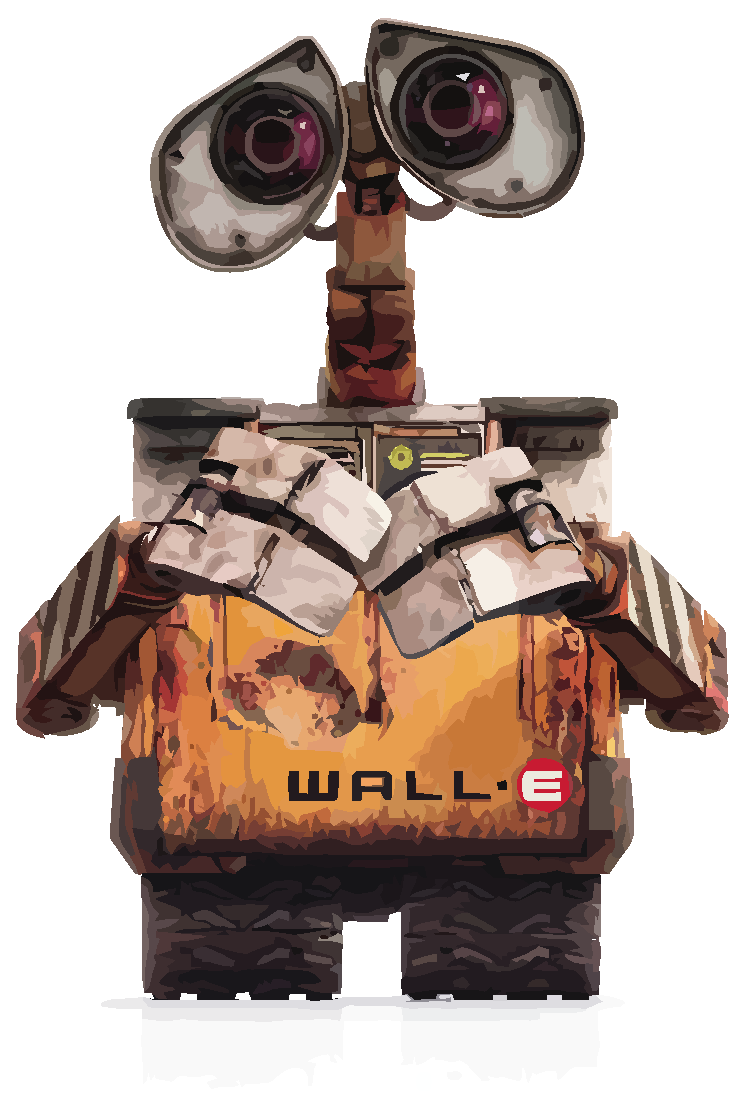
\includegraphics[width=\textwidth]{WallE}
    \caption{Wall-E}
    \label{fig:WallE}
  \end{subfigure}             
  \begin{subfigure}[b]{0.3\textwidth}
    
\includegraphics[width=\textwidth]{minion}
    \caption{Minions}
    \label{fig:Minnion}
  \end{subfigure}
  \caption{Best Animations}
  \label{fig:animations}
\end{figure}


\end{landscape}
\end{comment}
%%!TEX root = ../thesis.tex
%*******************************************************************************
%****************************** Third Chapter **********************************
%*******************************************************************************
\chapter{Research questions}

% **************************** Define Graphics Path **************************
\ifpdf
    \graphicspath{{Chapter3/Figs/Raster/}{Chapter3/Figs/PDF/}{Chapter3/Figs/}}
\else
    \graphicspath{{Chapter3/Figs/Vector/}{Chapter3/Figs/}}
\fi

\begin{itemize}
	\item How to proper model user behaviour in sequential decision making? In particular, how to design and learn the behavioural model when the user is interacting with a physical environment? (\textbf{RQ1})
	
	Motivated by the willingness to better understand users preferences in different contexts as well as to understand the influence of the presentation or consumption order of items we have to identify a suitable model that can learn the user preference from her action observations. As we discussed in the previous sections, typically users provides scarce feedback about the outcome of their action (i.e., if they liked or not to perform that action). Therefore, there is the need to identify a user behaviour learning solution that can cope with scarce this type of incomplete preference data. So far, we have experimented with an approach that ``groups'' similar users together (clusters) users and then learns, by means of IRL, a generalised user behaviour model that is specific to the group.  
	So far, we experimented with data that came from Location Based Social Networks (e.g., GPS traces of check-in actions). We will soon start to evaluate the proposed approach with sensor data coming from IoT devices.
	
	\item How can we use the learnt user behaviour model to generate more effective recommendations? (\textbf{RQ2})
	
	The next motivation of this study is that most of the current RS approaches do not distinguish between user behaviour learning and the recommendation  generation process. Current RS techniques (e.g., nearest neighbour) recommend items by identifying a user's choice pattern that is directly used to identify the set items the user is going to consume next. These are the items used for recommendation and often these recommendations are evaluated as too obvious for the target user.
	Therefore, we have to identify recommendation strategies that can be used in order to increase the user satisfaction rather than suggesting what the user is predicted to consume next. Furthermore, an aspect that have to be investigated is the presentation of the recommendations. In particular, in the case of Internet of Things scenarios we have to understand how to better address recommendation notifications to users.
	For instance, a user can be annoyed if he is notified every time a sensor identifies her presence close to items that are supposed to be relevant for her. Therefore, defining procedures to address this type of problems when dealing with IoT sensors is an important aspect of our research. 
	
	\item Quali sono i fattori che rendono una raccomandazione interessante per un utente ? (\textbf{RQ3})
	
	\item Which are the factors that make a recommendation interesting for a user? (\textbf{RQ4})

	\item It is possible to transfer the users' behavioural model learnt in a source domain to a target domain (\textbf{RQ5})?
	
	\item How do compare the recommendations generated by exploiting a source domain user behavioural model with those recommendation generated by harnessing the behaviour of target users (\textbf{RQ6})?
	
	
\end{itemize}

\begin{comment}

\section{First section of the third chapter}
And now I begin my third chapter here \dots

And now to cite some more people~\citet{Rea85,Ancey1996}

\subsection{First subsection in the first section}
\dots and some more 

\subsection{Second subsection in the first section}
\dots and some more \dots

\subsubsection{First subsub section in the second subsection}
\dots and some more in the first subsub section otherwise it all looks the same
doesn't it? well we can add some text to it \dots

\subsection{Third subsection in the first section}
\dots and some more \dots

\subsubsection{First subsub section in the third subsection}
\dots and some more in the first subsub section otherwise it all looks the same
doesn't it? well we can add some text to it and some more and some more and
some more and some more and some more and some more and some more \dots

\subsubsection{Second subsub section in the third subsection}
\dots and some more in the first subsub section otherwise it all looks the same
doesn't it? well we can add some text to it \dots

\section{Second section of the third chapter}
and here I write more \dots

\section{The layout of formal tables}
This section has been modified from ``Publication quality tables in \LaTeX*''
 by Simon Fear.

The layout of a table has been established over centuries of experience and 
should only be altered in extraordinary circumstances. 

When formatting a table, remember two simple guidelines at all times:

\begin{enumerate}
  \item Never, ever use vertical rules (lines).
  \item Never use double rules.
\end{enumerate}

These guidelines may seem extreme but I have
never found a good argument in favour of breaking them. For
example, if you feel that the information in the left half of
a table is so different from that on the right that it needs
to be separated by a vertical line, then you should use two
tables instead. Not everyone follows the second guideline:

There are three further guidelines worth mentioning here as they
are generally not known outside the circle of professional
typesetters and subeditors:

\begin{enumerate}\setcounter{enumi}{2}
  \item Put the units in the column heading (not in the body of
          the table).
  \item Always precede a decimal point by a digit; thus 0.1
      {\em not} just .1.
  \item Do not use `ditto' signs or any other such convention to
      repeat a previous value. In many circumstances a blank
      will serve just as well. If it won't, then repeat the value.
\end{enumerate}

A frequently seen mistake is to use `\textbackslash begin\{center\}' \dots `\textbackslash end\{center\}' inside a figure or table environment. This center environment can cause additional vertical space. If you want to avoid that just use `\textbackslash centering'


\begin{table}
\caption{A badly formatted table}
\centering
\label{table:bad_table}
\begin{tabular}{|l|c|c|c|c|}
\hline 
& \multicolumn{2}{c}{Species I} & \multicolumn{2}{c|}{Species II} \\ 
\hline
Dental measurement  & mean & SD  & mean & SD  \\ \hline 
\hline
I1MD & 6.23 & 0.91 & 5.2  & 0.7  \\
\hline 
I1LL & 7.48 & 0.56 & 8.7  & 0.71 \\
\hline 
I2MD & 3.99 & 0.63 & 4.22 & 0.54 \\
\hline 
I2LL & 6.81 & 0.02 & 6.66 & 0.01 \\
\hline 
CMD & 13.47 & 0.09 & 10.55 & 0.05 \\
\hline 
CBL & 11.88 & 0.05 & 13.11 & 0.04\\ 
\hline 
\end{tabular}
\end{table}

\begin{table}
\caption{A nice looking table}
\centering
\label{table:nice_table}
\begin{tabular}{l c c c c}
\hline 
\multirow{2}{*}{Dental measurement} & \multicolumn{2}{c}{Species I} & \multicolumn{2}{c}{Species II} \\ 
\cline{2-5}
  & mean & SD  & mean & SD  \\ 
\hline
I1MD & 6.23 & 0.91 & 5.2  & 0.7  \\

I1LL & 7.48 & 0.56 & 8.7  & 0.71 \\

I2MD & 3.99 & 0.63 & 4.22 & 0.54 \\

I2LL & 6.81 & 0.02 & 6.66 & 0.01 \\

CMD & 13.47 & 0.09 & 10.55 & 0.05 \\

CBL & 11.88 & 0.05 & 13.11 & 0.04\\ 
\hline 
\end{tabular}
\end{table}


\begin{table}
\caption{Even better looking table using booktabs}
\centering
\label{table:good_table}
\begin{tabular}{l c c c c}
\toprule
\multirow{2}{*}{Dental measurement} & \multicolumn{2}{c}{Species I} & \multicolumn{2}{c}{Species II} \\ 
\cmidrule{2-5}
  & mean & SD  & mean & SD  \\ 
\midrule
I1MD & 6.23 & 0.91 & 5.2  & 0.7  \\

I1LL & 7.48 & 0.56 & 8.7  & 0.71 \\

I2MD & 3.99 & 0.63 & 4.22 & 0.54 \\

I2LL & 6.81 & 0.02 & 6.66 & 0.01 \\

CMD & 13.47 & 0.09 & 10.55 & 0.05 \\

CBL & 11.88 & 0.05 & 13.11 & 0.04\\ 
\bottomrule
\end{tabular}
\end{table}
	
\end{comment}
%!TEX root = ../thesis.tex
%*******************************************************************************
%****************************** Third Chapter **********************************
%*******************************************************************************
%\chapter{User preference and behaviour learning in IoT augmented spaces}
\chapter{User preference and behaviour learning in physical spaces}
\label{cha:behaviour_learning}
% **************************** Define Graphics Path **************************
\ifpdf
\graphicspath{{Chapter4/Figs/Raster/}{Chapter4/Figs/PDF/}{Chapter4/Figs/}}
\else
\graphicspath{{Chapter4/Figs/Vector/}{Chapter4/Figs/}}
\fi


%%FR In generale in questo capitolo trovo molta descrizione dello stato dell'arte. Questo dovrebbe andare nel capitolo 2. Qui dovresti iniziare a descrivere i tuoi risultati.


\section{User-space interaction}
The underlying idea that motivates the research presented in this thesis is that RSs technologies can be employed not only to support people when they interact in the virtual world,
%%FR Io enfatizzerei meglio che tu usi dati collezionati sia analizzando comportamenti online che off-line per dare supporto sia online che offline. Qui dici solo che dai supporto quando agiscono off-line.
i.e., the web, but also when they act in physical environments, i.e., a city.
This is possible due to technological advancement in the field of sensing solutions, that brought novel possibility to capture human behavioural data in real environments, i.e., recording the offline user's behaviour. Sensed user behavioural data can then be leveraged to learn user's preferences. In this thesis we mainly focus on behavioural data acquired from sensors like GPS and IoT devices, such as, beacons.

\subsection{GPS data}
The GPS sensor on the mobile device of a user provides fine-grained location data that describes the mobility behaviour of the user. This information is typically formatted as a tuple $g=(lat,lon,t,\mu)$, where $lat$ and $lon$ are the latitude and longitude of the sensed location, $t$ is a timestamp and $\mu$ is the accuracy of the measure. A GPS device can update the location at the scale of seconds and can have an error in the range of few meters. 
%So, a user that moves and is equipped with a GPS sensor creates a trajectory of gps records. 
GPS data with different configurations of location updates and accuracy are used to support users in different scenarios: short interval location updates and high accuracy measures are typically used in navigation applications where the goal is to drive a user from location A to B in real time; non-frequent and less accurate locations updates are used in LBSNs 
%%FR esplicita l'acronimo
applications in order to identify locations of interest for a user.

%GPS data by nature lacks of semantic and therefore needs to be interpreted in order to use them in an application.
GPS data are by nature  noisy and therefore need to be processed in order to be used in an application.
The field of study that aims at extracting insights from GPS traces is trajectory data mining. 
%%FR puoi mettere un riferimento a proposito?
The term ``trajectory'' indicates the fact that a GPS device generates a trajectory %$\zeta_{gps} = (g_0,\dots,g_n)$ 
$\zeta_{GPS} = (g_j: j \in \{ 0, \dots, n\})$ 
%%FR non mi piace questa notazione. Io metterei (g_0, ..., g_n)
composed of $n$ location updates. In this thesis we adopt the following trajectory data mining techniques: stay point detection; trajectory segmentation; trajectory clustering; map matching. Stay point detection techniques are employed to identify the location, 
%%FR sembra, da quello che dici, che sia invece l'indentificazione del POI dai dati di location.
within a certain radius, where a user, or any moving objects, stayed for a given time-interval. A stay point can be, e.g., a restaurant or a museum that a user has been to, and, in addition to the GPS locations in a trajectory, it carries a deeper (semantic) meaning (i.e., it describes the user's action).
%%FR ??? Action? forse si potrebbe dire "intent". Ma questo dovrebbe derivare dalla letteratura e dalle definizioni che sono usate. Non credo che questo te lo sia inventato tu.
Trajectory segmentation methods deconstruct a trajectory into sub-trajectories by time interval, spatial shape, or semantic meanings. This representation is generated before performing clustering or classification. Map matching techniques aim at projecting trajectory GPS location onto the corresponding road segment where the point was generated.
%%FR metti appropriati riferimenti

The details of the trajectory data mining techniques that we employ/designed in order to process GPS data are detailed in Chapter \ref{cha:wondervalley}.

\subsection{IoT data}
IoT technologies make possible the exploitation of sensors networks to enable new ubiquitous information services \cite{iotdef:li,li:zhao:2015}. In fact, by distributing sensors in an environment or even by integrating them into objects it is possible to respond to user actions in real time as well as collecting data about the user behaviour \cite{iot:notifications, iot-sensor-healthcare, petrelli2013integrating}.
The IoT sensors that we consider for collecting human behavioural data are those that exploit  RFID, NFC and BLE short-range wireless technology. 
%%FR metti un riferimento ad un testo dove questi concetti sono spiegati. Espandi gli acronimi.
In contrast to GPS sensors, BLE allows to capture the actions a user performs as well as their semantic. 
%%FR ??? non capisco di cosa si tratti.

Peculiar to IoT augmented scenarios is the possibility to collect user physical actions data not only outdoor, but also indoor. For instance, by augmenting a physical space like the exhibition room of a museum (indoor) or a square in the old town of a city (outdoor) with a beacon device, i.e., small BLE devices broadcasting low-energy Bluetooth messages encoded with standard transmission protocols (e.g. Eddystone or iBeacon), is possible to collect user's behavioural data.
%%FR esemplifica
The broadcasted messages can be sensed by the Bluetooth receiver of the user mobile (smartphone) and, with the aid of background processes running on the devices, can fire the generation of location-based notifications or feed information to a user model in order to support further personalization of the system generated information
\cite{iot:beaconinteracton:Ng:2017}.
In addition, IoT augmented objects enable new possibilities to collect behavioural data about the user-space interactions. Sensors enabled objects allow to detect when they are moved and manipulated. This enable the possibility to design interactive scenarios where descriptive information about objects is presented to users at the very exact time when they are inspecting them, hence, stimulating enjoyment and sharing \cite{iot:tangibleinteraction:2009}.

We represent an interaction of a user with an IoT augmented place or object as a tuple $i=(id, a, t)$. With $id$ we denote the identifier of the IoT device with which the user interacted. The action $a$ performed by the user represent the semantic of the physical action, e.g., with ``visit'' we represent the visit to a POI or with ``play'' we mean the fact that a user started a media content. With $t$ we model the time (timestamp) at which the action $a$ is performed. 
%%FR ma non metti un id dello user?
Specific of user-IoT interactions is how the (geo) location information is handled: the $id$ of the IoT device can be used to enrich the record $i$ with information about the user location by using application domain knowledge, i.e., IoT devices are deployed in fixed positions of specific areas. Alternatively, the GPS of the user mobile device can be leveraged to annotate with the location coordinates the sensed interaction. The IoT traces of a user that who interacted $n$ times with the physical environment form a list 
%$\zeta_{IoT} = (i_0, \dots, i_n)$ 
$\zeta_{IoT} = (i_j : j \in \{ 0, \dots, n\})$ 
composed of actions updates (and locations) $i$.
In order to get more information about technical aspects about the IoT infrastructure that we have designed, in order to trace and respond to user's actions in sensor enabled spaces, we refer to our study ``Tangible Tourism with the Internet of Things'' \cite{massimo:enter2018}. 

\subsection{Social Network data}
Scientists in the fields of urban computing and computational social science have investigated how user behavioural data can be derived from social networks in order to investigate mobility and socio-economic aspects in specific geographical areas \cite{urban_computing:2014, urban_computing:LBSN:2019,eating_habits:lbsn:2014}.

LBSNs 
%%FR have you explained this acronym?
offer rich information about users' interactions in the physical space. For instance, in photo sharing platforms like Instagram\footnote{\url{https://www.instagram.com/}} each photo provides additional insight (e.g., descriptive tags, likes) about a location (geo coordinates) at a given time,
%%FR Ne sei sicuro? Non mi pare che in Istagram uno metta le coordinate delle foto. Qualche volta si specifica la locazione, ma non c'e' nessun controllo che la locazione immessa sia quella corretta.
whereas in check-in platforms like Foursquare City Guide\footnote{\url{https://foursquare.com/city-guide}} a location (e.g., a POI)
%%FR per te location e POI sono la stessa cosa? Per me un POI ha una location ma una location potrebbe non corrispondere ad alcun POI.
is enriched with metadata like the POI category (bar or shop) and opinions of the users (ratings or reviews).
Even though LBSNs offer such level of information about specific places in the physical environment, user's data are generally sparse if compared to the amount of data a GPS sensor can collect. % and, moreover, due to the structure of the platform is not easy to derive sequences of visited places for a specific individual.

Besides LBSNs, more traditional social networks, such as the photo sharing platform Flickr, offer the possibility to collect user behavioural data.
%%FR Cosa distingue Instagram da Flickr?
For instance, in \cite{indoor:lbsn:2018} Flickr\footnote{\url{https://flickr.com}} photos, their related geo data and tags have been used to identify indoor activities in the cities of New York and London. In other works \cite{danub:lbsn:2019} Flickr data has been used but never considering individual photos.
%%FR Non capisco cosa vuoi dire?
In \cite{lbsn:itineraries:2010} Flickr data have been leveraged in order to automatically generate visit itineraries. 

In this thesis we leverage Flickr data because its geo-localized pictures and their metadata are more likely to be related to the place where they have been taken. Moreover, since we are interested in learning users' preferences as well as their sequential decision making to generate next-item recommendations, we leverage Flickr data to retrieve individual sequences of observations.

For a specific user of a social network or LBSN a record can be represented as a tuple $l = (lat, lon, F, t)$, where $lat$ and $lon$ are the latitude and longitude of a location, $F$ is the set of features characterizing the location, e.g., the category of a POI or aggregate feedback expressed by the community on the POI, $t$ is the time at which the user added content to the LBSN platform.
%%FR quindi potrebbe essere molto diverso da quando quella location e' stata visitata. Dovresti discutere questi problemi.
For a LBSN user is possible to build a trajectory of the $n$ locations he was physically present %$\zeta_{LBSN} = (l_0, \dots, l_n)$.
$\zeta_{LBSN} = (l_j: j \in \{ 0, \dots, n\})$.
%%FR non si capisce bene queste locations da dove vengono. In realtà quello che l'utente fa e' di aggiungere dei contenuti o di creare dei post (cioe' fa delle azioni) da cui si deriva una location.

In this thesis we collect user behavioural data from the Flickr platform. In particular, from photo albums uploaded by users on Flickr, where each photo is geo-tagged, we reconstruct the itinerary a user followed.
%%FR Tutte queste discussioni sopra sono ancora descrizione dello stato dell'arte o di cose generali che non fanno parte dei tuoi risultati.

\section{Making sense of user-space interaction data}
\label{sec:user-space_mapping}
Either we have 
%%FR Non si capisce se stai facendo un discorso generale o se veramente tu adesso descrivi qualche tecnica e risultato costruito con questi due tipi di dati.
user-space interactions (trajectories) that have been collected by means of GPS sensor on the user mobile; sensed by the users' mobile Bluetooth receiver (interaction with a Beacon); or reconstructed from the user's profile on a social network, there is the need to build a representation of each interaction with the environment that allows to infer the underlying factors (preferences) that motivates the user's (offline) behaviour.

To attain this goal we need to employ a feature representation 
%%FR di cosa?
%can capture the latent behaviour in the data in such a way that a 
that a ML 
%%FR evita se puoi di usare acronimi. Qui hai spazio.
model can exploit to learn and generalize from the data. 
%%FR un modello e' addestrato o learned a partire dai dati. Non si capisce cosa vuol dire "generalize".
We think that for any scenario in which a user performs decision making 
%%FR che decisioni? Cerca di essere piu' specifico e non rimanere sul vago.
there are two main types of information that need to be considered: context information, describing what are the conditions in which the user operated; content information describing the items subject to the user's choices.

Let assume that any data trajectory $\zeta_{GPS}$, $\zeta_{IoT}$ and $\zeta_{LBSN}$ of length $n$ can be represented by a more general trajectory $\zeta = (o_j : j \in \{ 0, \dots, n\})$ where the user-space interaction observation $o = (lat,lon,t)$ models the fact that an interaction 
%%FR non dici che tipo di interazione? Non ti interessa distinguere? In quello che abbiamo fatto abbiamo sempre parlato di POI, stato e azione. Il POI e' una particolare locazione che ha uno specifico motivo di interesse, lo stato raccoglie altre informazioni legate al fatto che l'utente era nel POI in un particolare stato, e l'azione descrive quello che l'utente voleva fare, e' l'intent. Qui faccio fatica a trovare queste idee, che poi devi usare per descrivere i modelli. Si parla solo di locazione al tempo t.
happened at the location defined by the latitude and longitude pair $(lan,lon)$ at time $t$. With $O$ we denote the set of all the user-space interactions $o$. 
%%FR A me sembrano solo locazioni visitate da qualcuno, non specificato, al tempo t.
Let $E_{ctx}$ be the set of contextual informations in an external resource, 
%%FR Non c'e' bisogno di dire "external", da un punto di vista logico non ci interessa nulla sapere da dove vengono queste informazioni, se dal telefono o da un server o dal beacon ...
%% Inoltre non si capisce che tipo di spazio e' questo E_{ctx}.
%% Siccome dopo lo usi per dire che questo ti fornisce le "features" dello spazio degli stati, o qui o dopo devi descriverlo meglio. E' uno spazio R^n, e' {0,1}^n?
e.g., the content of a weather API, and let $E_{cnt}$ be the set of content information that can be obtained from an external resource, e.g., Wikipedia.
%%FR Stesso discorso. Queste abbiamo sempre detto che sono features del POI.
That said, in order to enrich with context and content data the observations in $O$, we have to identify two mappings: 
%%FR la prima cosa che devi mappare e'una location ad un certo istante in un POI. Le features sono features del POI non della location. Dal mio punto di vista. Se per esempio sei di fronte alla chiesa dei domenicani, sei alla chiesa dei domenicani o in piazza domenicani? Magari quella \psi_{cnt} che descrivi dopo potrebbe essere pensata come il mapping da una locazione fisica ad un POI.
$\psi_{ctx}: O \rightarrow E_{ctx}$ that maps a user-space interaction $o$ to a specific context, e.g., a POI-visit is mapped with its weather conditions; the mapping $\psi_{cnt}: O \rightarrow E_{cnt}$ that maps the same user-space interaction $o$ with content information, e.g., a POI-visit is mapped to its category.

The external information resources to be employed in order to enrich the user-space interactions observations can be: (1) generated (or defined) by domain experts; (2) identified among available online resources, e.g., Wikipedia.
For instance, in order to obtain content information in the tourist domain, with the objective of learning tourists' preferences, Wikipedia and Tripadvisor can be used as external resources.
With regard to context information, it is possible to derive relevant features directly from the user-space interaction data. For instance, the crowdedness of a place can be inferred from the geo-coordinates and the time recorded in the data: by defining a bounding geographic area, all the users that interacted at a specific time in that area provides the information about the size of the crowd. For other type of context data, like the weather, online resources can be used.

Here we describe an example showing how we add, by using Wikipedia data, content and context information to trajectories of visited locations in a city.
Content data falling within a geographic (bounding-box) area, defined by the minimum and maximum values of the $(lat,lon)$ pairs in the data, is retrieved from the external information source. %For instance, for a user trajectory of visited locations derived from a LBSNs the external source of information can be Wikipedia. 
%All the geo-localized Wikipedia pages that falls in the bounding box derived from the users' trajectories, minimum and maximum values of the $(lat,lon)$ pairs in the data, can be downloaded and then processed to identify a set of features, e.g., the place name and its type (bar or shop), to represent the location. 
Then, the retrieved content is processed to identify a set of features, e.g., the place name and its type (bar or shop), to represent the location. 
Afterwards, each location in a trajectory can be enriched with the identified content. In this way a pair of geographical coordinates becomes a recognizable POI and the trajectory becomes the itinerary of POI-interactions the user made in the physical space. From such, richness of information in the data user behaviour information can be learnt.

\section{Learning a user preference model}
\label{sec:learning_user_preferences}
In this section we detail how we learn user's preferences and behaviour from observed user-space interaction trajectories.
In particular, we present how we model the problem of the trajectory generation task, which is closely tight to the problem of sequential decision making. Afterwards, we detail how we  learn user' preferences as well as her action-selection policy. 

\subsection{Problem modelling}
%\textbf{Markov Decision Process Model.} 
We model the user-space interaction trajectory generation task
%%FR Non sono convinto che questo risolve in "generation task". Devi aver gia' generato le trajectories per costruire il tuo MDP. MDP e' il modello formale in cui sistematizzi il problema decisionale dell'utente, non le traiettorie, che sono delle sequenze di azioni.
as a finite Markov Decision Process (MDP). A MDP is defined by a tuple $(S,A,T,r,\gamma)$. With $S$ we denote a finite set of states and in our scenario a state represents the interaction of a user with the physical space (e.g., visiting a POI) in a specific context (e.g., weather, temperature and day). For instance, a tourist that visits the old town of Florence can be at the Battistero (POI) in a cloudy, cold morning (context). $A$ is a finite set of actions, which in a tourism scenario can represent the decision to move to a POI. With $T$ we indicate a finite set of probabilities $T(s'| s, a)$, to make a transition from state $s$ to $s'$ when action $a$ is performed. For example, a user that visits Battistero in Florence during a cloudy morning (state $s_1$) and wants to visit the Uffizi Gallery (action $a_{1}$) in the afternoon can arrive to the desired POI with either a cloudy sky (state $s_2$) or a clear sky (state $s_3$) with transition probabilities $T(s_2,a_{1}|s_1)=0.5$ and $T(s_3,a_{1}|s1)=0.5$.
The function $r: S \rightarrow \mathbb{R}$ models the reward a user obtains from visiting a state. This function is supposed to be {\it unknown} and must be learnt, i.e., we take the restrictive assumption that we do not know the utility the user receives from her interaction with the environment (the user is not supposed to reveal it). But, we assume that if the user performed an action and not another one, then she believes that the first action gives her a larger utility/reward than the second. Finally, $\gamma \in [0,1]$ is used to discount future rewards with respect to immediate ones. 
%
We denote with $\zeta_u$ a user $u$ trajectory,
%%FR Lo avevi fatto anche prima ma le traiettorie erano prima sequenze di locazioni. Devi evitare questa confusione. Hai troppi di tipi di traiettorie. Magari puoi distingure tra traiettorie di locazioni e traiettorie di stati. Le prime sono le osservazioni fisiche e le seconde sono arricchite da altre informazioni (contesto, intent dell'utente, features del POI, ecc).
which is a temporally ordered list of state-action pairs (user-space interactions). 
%%FR In un MDP si parla di sequenze di stati non di stati-azione. Hai davvero bisogno di parlare di stato-azione. Noi abbiamo sempre inteso che lo stato descrive anche l'azione, ovvero se un utente e' in un POI vuol dire che voleva visitare questo POI. Non abbiamo casi in cui un utente voleva visitare il POI a e si trova invece al POI b. Puoi lasciare stato-azione ma se non serve crea solo confusione.
For instance, $\zeta_{u_1} = ((s_{10},a_{3}), (s_5,a_8), (s_{15}, a_e))$ represents a user $u_1$ trajectory starting from state $s_{10}$, moving to $s_5$ by performing action $a_3$ 
and ending to $s_{15}$ by acting according to $a_8$. The last action $a_e$ is a dummy action that indicates the end of the trajectory. With $Z$ we represent the set of all the observed users' trajectories. 
%
Given a MDP, our goal is to find a policy $\pi^* : S \rightarrow A$ that maximises the cumulative reward that the decision maker obtains by acting according to $\pi^*$ (optimal policy). 
The value of taking a specific action $a$ in state $s$ under the policy $\pi$, is computed as :

$$Q_{\pi}(s,a)=\mathbf{E}^{s,a,\pi}[\sum_{k=0}^{\infty} \gamma^k r(s_k)]$$

i.e., it is the expected discounted cumulative reward obtained from $a$ in state $s$ and then following the policy $\pi$.

%\begin{equation}
%\label{eq:bellman} 
%Q_{\pi}(s,a) = \sum_{s'}T(s'|s,a)r(s')+\gamma \max_{a'}{Q_{\pi}(s',a')}
%\end{equation}

The optimal policy $\pi^*$ dictates to a user in state $s$ to perform the action that maximizes $Q_{\pi^*}$. So, in order to compute $Q_{\pi^*}$ we rewrite the previous formula as:

$$Q_{\pi^*}(s,a) = \sum_{s'}T(s'|s,a)\left[r(s)+\gamma \max_{a'}{Q_{\pi}(s',a')}\right]$$

%%FR sei sicuro di questa formula? Il Q tra parentesi non e' relativo a pi^*? Non e' la formula di Bellman?

The problem of computing the optimal policy for a MDP is solved by Reinforcement Learning algorithms \cite{sutton:1998}.

As we mentioned earlier, in a information systems and specifically in RSs applications the reward obtained by a user when she is in a specific state (i.e., the $r$ function) is usually unknown because users scarcely provide feedback (e.g., ratings or reviews about the consumed items). Therefore, we are interested in determining the reward function $r$ from the bare observations of the decision maker transitions from state to state; this problem is solved by Inverse Reinforcement Learning (IRL). 


\subsection{IRL}
%%FR Secondo me queste cose generali su MDP e IRL andrebbero nello stato dell'arte e qui dovresti spiegare come lo hai applicato al nostro dominio. Ora magari e' troppo complesso separare. Ma dovresti cercare piano piano di sposatre nello stato dell'arte le cose generali in modo che qui la discussione e' davvero specifica.
IRL algorithms take as input a model of the environment, the MDP, and the observed behaviour of a user (or any autonomous agent) in the form of demonstrations, in our case the trajectories in $Z$,
%%FR Le traiettorie di stato o di stato-azione?
and return the inferred user's reward function. In IRL the underlying assumption is that a user is a rational decision maker who seeks to optimize the reward associated to her actions. Due to this, the agent is typically referred as ``expert''.

Generally the state space $S$ is represented by a state feature function $\Phi:S \rightarrow \mathbb{R}$ that assigns to each feature a real value.
%%FR ??? Questa sara' una funzione in R^n non in R perche' uno stato e' descritto da molte features non una.
We model each state by using the features identified with the mappings $\Psi_{cnt}$ and $\Psi_{ctx}$ (Section \ref{sec:user-space_mapping}).
%%FR Come dicevo prima, devi spiegare meglio che tipo di spazio e' questo e magari fare un esempio concreto che aiuta a capire.
%For instance in the tourism domain a reasonable set of state features that can be used to infer the reward a tourist obtains from observations of POI-visit, can be: the type of a POI; opening hours; the weather; the day of the week; amount of visitors; the price range. 


In order to infer the user's reward from her observations there is the need to identify a solution, i.e., a reward function, that makes the observed behaviour optimal. 
IRL algorithms can reconstruct the reward function $r$ and the optimal action-selection policy $\pi^*$ of a user $u$ from the set of her observed trajectories. We assume (as in \cite{ng:2000}) that $r$ is a linear function, $r(s) = \theta^T\phi(s)$, of the state $s$ feature vector $\phi(s)$ 
%%FR perche' ora la funzione che produce le features e' phi minuscolo e prima era Phi maiuscolo?
and the user utility vector $\theta$, which models the unknown user preference for the state features. IRL algorithms derive the user's action-selection policy from the learned reward function $r$ by assuming that users act in order to maximise the reward.

Researchers in the field of IRL showed that the reward estimation problem is ill-posed because there is an infinite number of solutions, e.g., a reward function $r=c$, where $c$ is a constant, is an example of such problem.
%%FR Non si capisce cosa vuoi dire. Che se la reale funzione di reward e' una costante allora qualunque funzione costante e' anche una soluzione? Spiega meglio.
Therefore, the challenge in IRL is to seek for a solution that is optimal, the best among the set of all the solutions. 
%%FR Cosa vuol dire "the best"? Il problema che hai descritto sopra e' che non esiste UNA best, ma ne esistono MOLTE e che non si puo' dire qual'e' quella che l'utente sta realmente usando, assumendo che lui ne usa una sola.
The main difference among the IRL algorithms proposed in the literature is in how the solution is computed, i.e., they differ in the optimality criterion.
%%FR Quindi? Ne trovano una tra le tante soluzioni ottime? Vuoi dire questo? Sembra qusi che dici che hanno diversi criteri di ottimalita'. Questo e' fuorviante. Trovano diverse funzioni di reward che pure determinano la stessa policy ottima.

To resolve the issue of identifying an optimal solution in \cite{ng:2000,irl:optimal_solution:2006} has been proposed to add a margin in order to maximize the difference between the reward derived from the optimal policies an the reward that is derived from the alternative policies.
%
In \cite{bayesianIRL} the authors tackle the problem of computing the reward from a Bayesian perspective. The proposed model, called Bayesian IRL, leverages the users' observations in order to infer the optimal reward. At first, it uses the observations as evidence to update the prior knowledge on the set of possible reward functions (solutions), which are assumed to be independently identically distributed. Then, Bayesian IRL estimates the reward using the posterior knowledge.
%
The authors of Maximum-Entropy IRL \cite{maxentirl} propose to seek for a reward function by matching state features in the observation data. Maximum-entropy is used to identify action (i.e., user-space interactions in our case) probabilities that lead to a reward that supports the observed data.
%%FR Queste sono cose generali che andrebbero messe nello stato dell'arte su RL e IRL. Qui interrompono la discussione specifica alla tua applicazione.

\subsection{Maximum Log-Likelihood IRL}
In this thesis, in order to learn both the user's reward and her action-selection policy, we use a specific IRL algorithm called Maximum Log-likelihood (MLIRL) \cite{vro:litt:2011}. 
MLIRL combines many positive features of other IRL models \cite{bayesianIRL,maxentirl,policymatchingirl}: it assumes a prior knowledge of the user preference vector to estimate an initial reward function that is then adjusted by looking for a maximum likelihood model that can justify observed trajectories; it optimizes user behaviour via a gradient method and assumes that each user randomizes the action selection process at the level of individual choices, i.e., by sampling choices (actions) from a Boltzmann distribution. 

%In MLIRL it is assumed that experts randomize individual action choices. Choice actions are sought by the maximum likelihood solution via the gradient ascent approach. 
The algorithm exploits the fact that a guessed $\theta$ induces a probability distribution over action choices and hence determine a likelihood for the observations in $Z$. Expected values (discounted) are computed via the following formula:
% Add Bellman equation somewhere before

%\begin{equation}
$$Q_\theta(s,a) = \theta^T\phi(s)+\gamma\sum_{s'}T(s,a,s')\frac{\sum_a Q_\pi(s,a)e^{\beta Q_\pi(s,a)}}{\sum_{a'}e^{\beta Q_\pi(s,a')} }$$
%\end{equation}

MLIRL looks for $\theta = \arg\max_\theta L(Z|\theta)$ which is the maximum likelihood solution that is found via gradient ascent optimisation. 
The log likelihood of the observed trajectories $Z$ is defined as:

%\begin{equation}
$$L(Z|\theta) = \prod_{i=0}^{|Z|} \prod_{s,a \in \zeta_i} \pi_\theta(s,a)$$
%\end{equation}

The term $\pi_\theta(s,a)$ in the previous equation represents the Boltzmann action-selection policy, which is defined as:

$$\pi_\theta(s,a) = \frac{\sum_a Q_\pi(s,a)e^{\beta Q_\pi(s,a)}}{\sum_{a'}e^{\beta Q_\pi(s,a')}}$$

The computation of $\theta$ via gradient ascent is performed for a fixed number of steps $M$. At each step the $\pi_\theta(s,a)$ is computed by solving via value iteration the MDP, using the estimated reward $r(s) = \theta^T \phi(s)$.

MLIRL is known to converge to a solution in finite-horizon settings and is also known to produce a well-defined answer. The problem of the existence of multiple reward functions for which an observed trajectory is optimal in a given MDP, is solved by assigning high probabilities to observed behaviour and low probability to the unobserved. The general steps of the code are listed in algorithm \ref{code:mlirl}.

\begin{algorithm}
	\caption{Maximum Likelihood Inverse Reinforcement Learning}
	\label{code:mlirl}
	\begin{algorithmic}
		\State \textbf{Input:} S, A, T, $\gamma$, $\phi$, $Z=\lbrace \zeta_1, \dots,  \zeta_N \rbrace$, M, $\lambda_t$ step size.
		
		\State $\theta \leftarrow$ Initialize with random values;
		\For{t=1 to M} 
		\State Compute $Q_{\theta_t}$,$\pi_{\theta_t}$
		\State $L = \sum_{i} \Pr{(\zeta_i)} \sum_{(s,a) \in \zeta_i} \log{\pi_{\theta_t}(s,a)}$
		\State $\theta \leftarrow \theta + \lambda_t\nabla{L}$
		\EndFor
		\State \textbf{Output:}  $\theta$
	\end{algorithmic}
\end{algorithm}

\section{Learning from scarce individual's behavioural data}
\label{sec:clustering like behaving users}
%Finally, we show how the problem of learning an individual behaviour model from scarce user behavioural data, a common problem in information systems, can be alleviated by clustering trajectories of like-minded users and then learning a (one per cluster) generalized behavioural model.

As we have shown in the previous section by harnessing behavioural data of an individual, i.e., user-space interaction trajectories, we can learn with IRL the user behavioural model in terms of the user's preferences $\theta$, her reward $r$ and the associated action selection policy $\pi^*$. 
%%FR Non e' che questo lo hai mostrato bene. Hai descritto MDP, hai detto che con IRL puoi stimare la reward, hai forse detto che con la reward function uno puo' calcolare anche la policy ottima. Secondo me tutto questo e' poco chiaro. Non hai mai mostrato esempi e hai mescolato cose generali a cose specifiche. Secondo me le cose generali su RL e su IRL andrebbero nello stato dell'arte e magari con degli esempi classici per far capire cosa succede in quei casi. Qui dovresti solo focalizzarti sul tuo caso specifico e far capire come queste tecniche generali sono state utilizzate da te.

Generally, in information systems 
%%FR cosa sono questi "information systems"? Cerca di essere piu' specifico. Tu ti sei occupato di una particolare applicazione nell'ambito del turismo. Parla di quello se no uno come fa a capire a cosa ti riferisci?
the amount of individual user behavioural data is not large for the majority of the system users. The lack of user's data becomes more evident when it comes to user-space interaction data, for which the available public datasets are not many (and sparse as well) and the only rich datasets are those owned by service providers like Google, Foursquare, and Uber.
%%FR Io direi le cose in modo diverso, altrimenti sembra che tu abbia sviluppato una tecnica solo perche' non hai accesso ai dati. Devi valorizzare l'idea del clustering piuttosto che descriverla come un ripiego.
We think that from a RSs perspective, which is the focus of this thesis, using only target user (specific) behavioural data
%, even a rich set of individual data, 
for recommendations generation for him is of scarce utility for the user: 
%%FR in realtà nessun RS, a parte quelli content-based, usa solo i dati del target user per fare raccomandazioni a lui. In CF si usano i dati di una popolazione di utenti.
the suggested items (e.g., POI-visits) will (probably) be those that the user would choose without the help of the RS. 
%%FR E' il tipico problema dei CB RSs.
Moreover, individual behavioural data may present a sub-optimal behaviour. e.g., a user that visits for the first time a city may simply visit the few, more accessible, places that are closer to the city main attractions. Learning a behavioural model from such observations would lead to a biased model. We think that by learning, instead, a behavioural model from observations of more visitors 
%%FR ma devi dire cosa vuol dire "more" in questo contesto.
in the city, the resulting learnt behaviour will minimize the impact of sub-optimal behaviours that could influence some of the observed trajectories.

In order to alleviate the problems of learning from scarce user's data and minimizing the impact of suboptimal behaviours present in the data, we propose to group the user-space interaction trajectories in clusters and then to learn a ``general'' user behavioural model common for all the users/trajectories in a cluster.

By applying MLIRL on each cluster of trajectories we therefore learn cluster specific reward functions and behaviour models of the users in each cluster. This is the optimal policy that dictates for each state the best action, e.g., the next POI visit, the users in a cluster should take in order to maximise their reward.

%\subsection{Alleviating the problem of scarce individual users' interaction data via clustering}
\subsection{Clustering like-behaving users}
Clustering the trajectories is implemented 
%%FR Dove???? Non si capisce chi lo fa questo.
with Non Negative Matrix Factorization (NMF)
\cite{nmf:majorcontribution:1999}, which is a specific class of Matrix Factorization models. Matrix Factorization has the objective of reducing an input matrix into its constituent parts in order to ease the computation of more complex matrix operations or inspect the input data. 

Applications of NMF can be found in many field of science, e.g., in astronomy, NMF is used to process space observation data in order to identify planets that cannot be directly observed due to the high amount of light that stars close to the planet emits \cite{nmf_astronomy:2018}; in biology, NMF has been used to cluster gene expression \cite{nmf_biology:2012}. Of our interest is the application of NMF in text mining where NMF allows to group documents to a common semantic structure that can explain the resulting clusters.
%%FR Spiega quali sono i documenti che usiamo noi.

NMF requires as input a positive real valued matrix, therefore documents needs to be represented by using an appropriate statistic, i.e., term frequency–inverse document frequency (tf-id). Given a set of documents, i.e., a text corpora, the tf-idf statistic represent numerically how important is a term in a document. Let $d \in C$ be a document belonging to the corpus $C$ and let be $t \in d$ a term of the document. The tf-idf is computed by means of the following formula:
%%FR di nuovo roba generale che andrebbe nello stato dell'arte.

$$tfidf_{d,C}(t) = tf_d(t) \cdot idf_C(t)$$

The term $tf_d(t)$ is the term frequency of the term $t$ for the document $d$; we compute it as 
%$tf(t,d) = \frac{\sum_{j\in d}\textbf{1}_{j,d}}{|d|}$. The indicator function $\textbf{1}_{t,d}$ has value 1 if the term $t$ is present in document $d$, otherwise 0. 
$tf_d(t) = \frac{count_{d}(t)}{|d|}$. The numerator $count_d(t)$ is the number of terms in $d$ that are equal to $t$. 
%%FR e il denominatore?
%% Ma non usi anche qui il logaritmo della frequenza? 

The second term in the formula is the inverse document frequency $idf_C(t)$ and express how much a word is important, i.e., a word is rare or common in the corpora $C$. We compute it as:
%%FR non e' che lo calcoliamo noi cosi', questa e' una definizione generale.

$$idf_C(t)=log \frac{|C|}{|d\in C: t\in d|}$$ 


In order to use NMF to identify like-behaving/minded users from their user-space interactions trajectories we need to build a document-like representation of the trajectories. To generate such representation we harness (for each trajectory $\zeta$) the mappings $\Psi_{cnt}$ and $\Psi_{ctx}$ that we defined in Section \ref{sec:user-space_mapping}. We recall that these mappings identify descriptive features for each user-space interaction in the data. 
%%FR qui intendi per features delle keywords, ovvero il valore delle features. Penso. E' difficile dire perche' prima non descrivi bene le funzioni che mappano una locazione in un contesto o in un contenuto.
For instance, if the user visited a museum the descriptive features associated to the interactions can be: content information describing the visited place, e.g., the type of museum (science), the exhibition style (interactive); context information, e.g., the part of the day (afternoon), the weather (rainy) and the crowdedness of the place.
By representing each observed user-space interaction with its associated features (terms), we generate a document that describes the observed interaction of the user with the environment. When this operation is performed by using all the trajectories in the database we obtain the corpora that describes the interactions of all the users. 

With $D$ we denote the tf-idf matrix representation of the obtained corpora.
%We denote with $D$ the \textit{tf-idf} matrix representation of the obtained corpus. 
Columns in $D$ represents specific terms and rows corresponds to trajectories. 
The matrix $D$ has size $|Z| \times F$, where $F$ is the number of unique terms in the corpora. NMF approximates the matrix $D$ with the product of two non-negative matrices $W$ (of size $F \times K$) and $H$  (of size $|Z| \times K$).
%%FR Ma allora sara' HW^T. Scrivi la formula di approssimazione se non non si capisce cosa dici.
The matrix $H$ identifies which topics (columns) are more relevant for each user trajectory (row), and using it we assigned a trajectory to the topics that in its corresponding row have values larger than a threshold $\tau$ as similarly done in \cite{nmf:multilabelannotation:2017}. Hence, each topic defines a cluster of trajectories.
Moreover, a topic, can be described by its top terms, i.e., those with the largest values in the corresponding row in $W$.

In order to identify the correct number of topics (clusters) we conduct  a stability analysis, as suggested in \cite{topicmodeeling:greene2014}.
The procedure seeks for the best number of topics $k$ from a pre-defined space. At first, a reference $k$-topic model $M^{ref}$ is generated by using the whole corpora.  The reference model $M^{ref}$ comprises the lists of $m$ top terms of each topic. Then, a fixed number of documents subsets are sampled (without replacement) from the corpora. 
%%FR Ma quando spieghi quello che hai fatto tu???? Questa sembra ancora roba generale.
%% Qui devi descrivere per filo e per segno quello che hai fatto, non solo le tecniche generali.
%The reference model $M_{ref}$ comprises the lists of $m$ top terms of each topic and is used to assess the stability of the topics generated by corpora subsets for different $k$ values.
For each documents subset $G_i$ we generate the $k$-topic models $M$ and compute the agreement between the reference model $M^{ref}$ and $M$. With $\mathcal{M}$ we denote the set of $k$-topic models built from $G_i$. The computation of the agreement between two $k$-topic models is performed by: (1) building a square matrix $J$ containing the average jaccard values of the $k$ topics in $M^{ref}$ (rows) and the $k$ topics in $M$ (columns); (2) computing the agreement score $agree(M^{ref},M)$.

In particular, the average jaccard score for the $k$-th topic, with $m$ top words, in $M^{ref}$ and $M$ is computed using the formula:

$$\overline{jacc}(M^{ref}_{k}, M_{k}) = \frac{1}{m} \sum_{l=0}^{m} \frac{|M^{ref}_{k,l} \cap M_{k,l}|}{|M^{ref}_{k,l} \cup M_{k,l}|}$$

The agreement score for the 
%$$agree(M^{ref},M)=\frac{1}{k} \sum_{i=1}^{k} \overline{jacc}(M^{ref}_{k}, best_{\overline{jacc}}(M_{ref,k},M_{i,k})) $$

$$agree(M^{ref},M)=\frac{1}{k} \sum_{i=1}^{k} \max{J_k}$$

Finally the stability is computed as:

$$stability(k) = \frac{1}{|G|} \sum_{i=1}^{|G|}agree(M^{ref},\mathcal{M}^i)$$

The best number of topics/clusters $k$ is the one with highest stability score (mean agreement).
%%FR ma non si capisce come cerchi nello spazio di tutti i possibili k. Hai detto che parti da un k e non dici che valore ha, e poi non dici quali altri valori di k provi.

\section{Case study: Learning user preferences and behaviour in open spaces}
%%FR Io non lo presenterei come "case study" se no sembra solo che tu hai fatto un case study con tecniche ben note. Se presenti le cose in questo modo togli valore al tuo lavoro.

%In ``L'' \cite{} we show an example of learning user's behaviour in an indoor IoT augmented space.
In this case study we present how user-space interaction data can be leveraged to learn tourists' behaviour in the scenario of visiting a cultural heritage centre. %User's visit actions trajectories are acquired from the Flickr photo sharing platform and additional content and visit context information have been retrieved from Wikipedia and a weather API.

\subsection{Available data}
The dataset we employ consists of 1663 users' POI-vist trajectories in the city of Florence (Italy) that have been reconstructed by employing data harvested from the Flickr photo sharing platform.
%%FR ma non l'hai fatto tu. Devi dire chi ha fatto cosa in maniera chiara.
%Tourists' offline behavioural data have been retrieved from the Flickr\footnote{https://flickr.com} photo sharing platform.
The POI-visit trajectories are built by following the general example presented in Section \ref{sec:user-space_mapping}.
In particular, images in a Flickr photo album are tagged with information about the geographical coordinates and the shooting time, from these information a trajectory 
%%FR prima hai dato diverse definizioni di traiettoria. Cos'e' ora una traiettoria? Usa le definizioni che hai dato.
is constructed as follows: (1) geographical coordinates are used to represent the picture as a recognizable POI by fetching relevant content data from an external source; (2) the shooting time is used to order the identified POIs in such a way that we obtain a temporally ordered list of user's visited POI, i.e., the user itinerary. 
%%FR Ma non puoi ora descrivere ora con precisione le varie funzioni che hai descritto sopra e che fanno parte del tuo modello generale?
So, photo albums which elements fall within the geographical boundaries of the city of Florence\footnote{\url{https://www.openstreetmap.org/relation/42602\#map=12/43.7716/11.3291}} have been downloaded and sorted.
%%FR lo hai fatto tu?
Each photo is then matched with the Wikipedia pages whose geographical coordinates fall within the Florence area. The matching procedure is done by defining a circular area, with fixed radius ($r=100$ meters), centred in the photo coordinates and then by seeking  for the closest Wikipedia content geo-localized in that area.
In this case study we use as starting point the POI-visits trajectories dataset presented in \cite{flikr_tourism_RS:muntean:2015}.
%%FR quindi il match lo hanno fatto loro? Devi essere piu' preciso nel dire quello che hanno fatto loro e quello che hai fatto tu.
We manually added to each POI-visit data content information about the POI itself by using expert knowledge extracted from the POI Wikipedia page. Since all the identified POIs are cultural attractions we decided to identify the following set of features to represent them: 
%%FR questo lo devi descrivere bene e motivare perche' ha un impatto notevole sul modello comportamentale.
the POI category (e.g., monument), the historical period (i.e., century) and one historical person related to the POI. In the 532 POIs appearing in the trajectories we identified 13 different POI categories, 18 historical periods and 106 historical persons. 
With regard to the visit context of a POI-visits we leveraged the timestamp (the date) and the geographical coordinates of each POI-visit to query a weather service\footnote{\url{https://darksky.net}} to collect an hourly weather summary (e.g., cloudy), temperature (e.g., cold) and daytime (e.g., evening). 
%%FR Anche questo deve essere motivato meglio perche' ha un impatto sul modello comportamentale che poi apprendi.

The trajectories/users ratio is 1.43 and the average trajectory length is 11.7 POI-visit. 
%%FR e cosa vuol dire questo? Spiega, commenta.

\subsection{Identification and inspection of like-behaving users}
In order group like-behaving users in the dataset we apply the approach described in Section \ref{sec:clustering like behaving users}. So, we generated a text corpora by building a document-like representation for each trajectory. The terms in the corpora are the content and context features associated to the POI-visits. Then, we applied NMF and we identified 5 different trajectory clusters.
In Table \ref{tab:Topics} we show the top-10 terms per cluster and the number of associated trajectories. Clusters are named with the first 5 English alphabet letters.

\begin{table}[h]
	\centering
	
	\caption{Top 10 terms in the five topics extracted from the trajectory data set and number of trajectories assigned to each topic (cluster).}
	
	\label{tab:Topics}
	\begin{tabular}{ |l|l|l|l|l|l| }
		\hline
		\textbf{\#Term} & \textbf{Cluster A} & \textbf{Cluster B}  & \textbf{Cluster C}& \textbf{Cluster D} & \textbf{Cluster E}  \\ \hline
		1  & morning &hot &cloudy &warm &freezing   \\ \hline
		2  & cold &afternoon &cold &cloudy &cloudy   \\ \hline
		3  & square &century 16 &church &century 14 &afternoon   \\ \hline
		4  & palace &palace &square &church &century 14   \\ \hline
		5  & century 15 &church &century 13 &square &palace   \\ \hline
		6  & century 13 &square &palace &building &building   \\ \hline
		7  & church &century 19 &rain &palace &century 13   \\ \hline
		8  & night &century 13 &museum &ponte &church   \\ \hline
		9  & dante &museo &brunelleschi &century 13 &foggini   \\ \hline
		10 & century 10 &brunelleschi &tadda &century 19 &century 19   \\ \hline
		\hline
		\textbf{\#Traj.} & 368 & 339 & 341 & 297 & 153 \\ \hline
		
	\end{tabular}
\end{table}

In the following, we exemplify the results of the clustering step by comparing two cluster examples (i.e., C and E); they have some similar features but a different number of trajectories. Figure \ref{fig:cluster_map} depicts the clusters' trajectories and 15 most popular POIs.

\begin{figure}
	\centering
	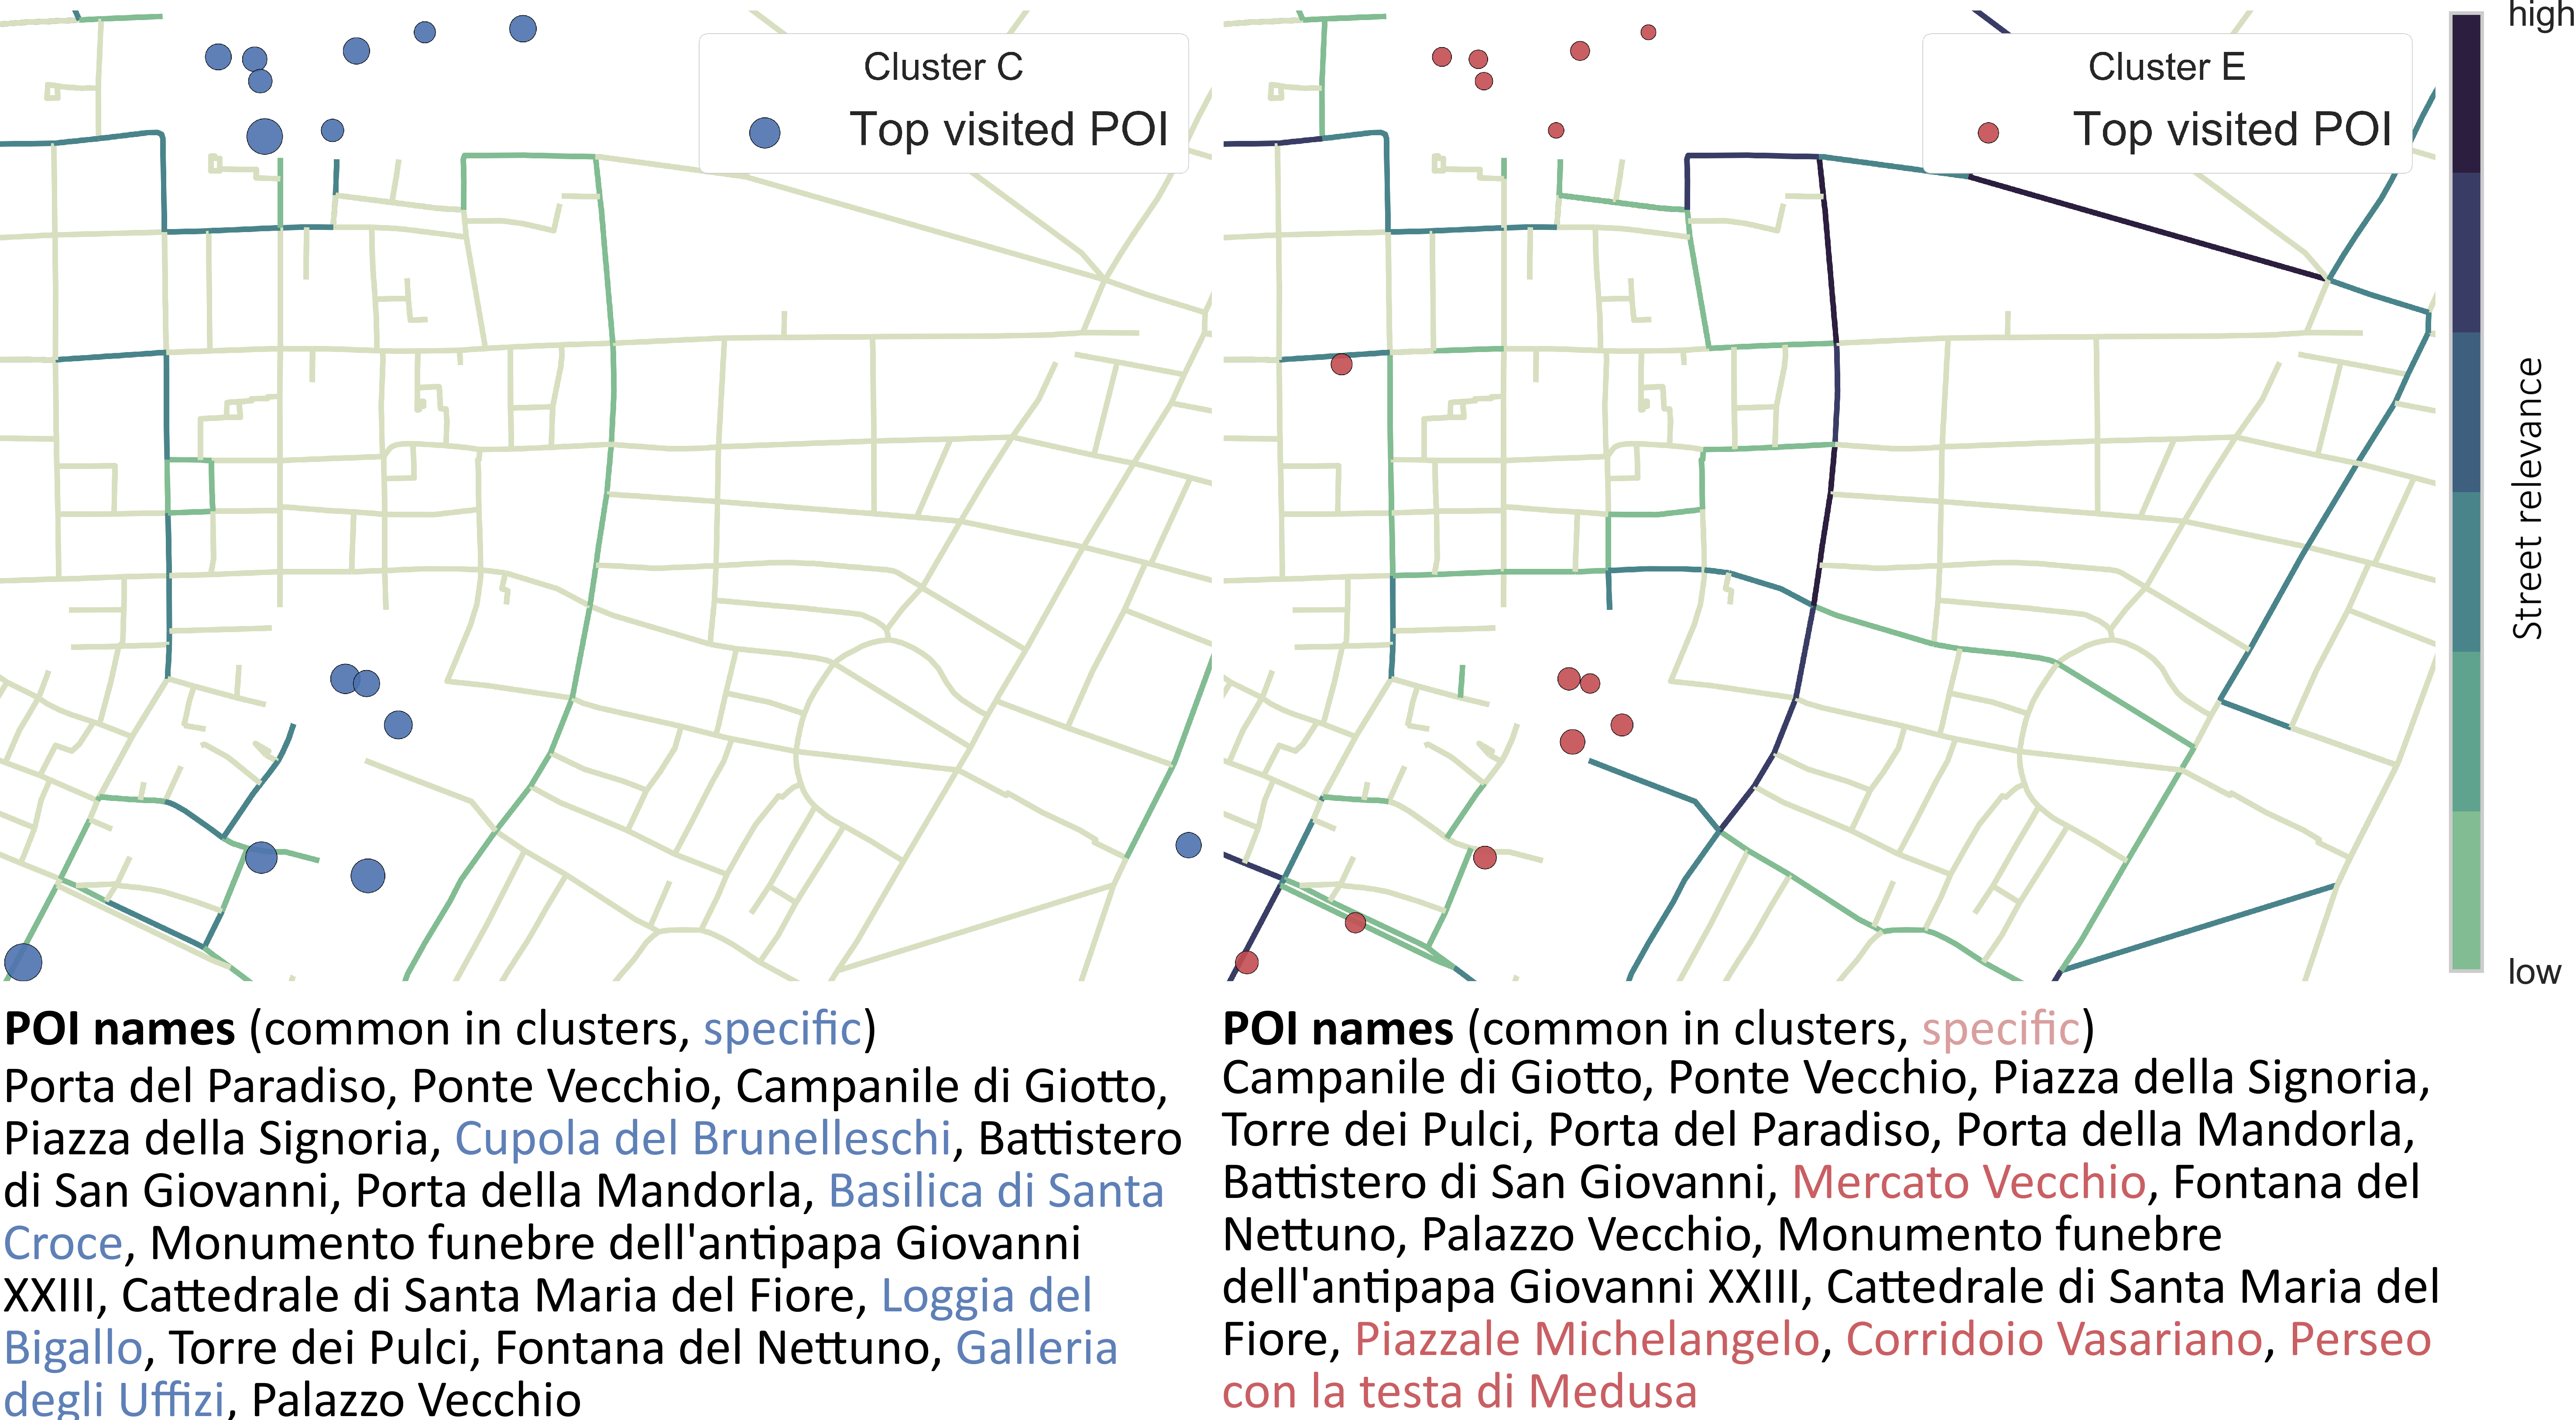
\includegraphics[width=\linewidth]{cluster_comparison_poinames}
	\caption{Top-15 visited POIs and street relevance (heatmap) for two clusters}
	\label{fig:cluster_map}
\end{figure}

The POIs are depicted as circles with diameter proportional to the normalised POI popularity:  the more popular the POI is in the cluster the larger the circle is. There is a large number of POIs present in both clusters, but they differ in terms of normalised visit frequency. In fact, in the cluster represented on the right (cluster E), POI circles are smaller because of a more uniform distribution of the visits among all the POIs in the cluster (i.e., not only the top-15 shown in the figure). 
An aspect that we see of particular interest is related to how users interacts with the surrounding environments. To show that, in Figure \ref{fig:cluster_map} we show how important are the streets of Florence for the clustered users/trajectories.
The importance of the various streets in the clustered trajectories is determined by identifying the most representative trajectories in the clusters. These are the trajectories whose \textit{tf-idf} vector representation is closer, in cosine similarity, to the cluster centroid, which is the average vector of all the \textit{tf-idf} vector trajectory representations. The street importance is represented as shades of the colour bar on the right part of the figure; it has higher values (darker colour) in proximity to popular POIs and on the main streets connecting them. 

At the bottom of Figure \ref{fig:cluster_map} the most popular POIs in the two clusters are listed. POI in black typeface are common to the two clusters, whereas coloured POIs are cluster specific. 11 POIs are common to these two clusters and 9 of them are common to all the clusters. They actually belong to the top-15 attractions according to popular travel portals\footnote{
	\url{www.planetware.com/tourist-attractions-/florence-i-to-f.html} \\  
	\url{www.touropia.com/tourist-attractions-in-florence/} \\ \url{theculturetrip.com/europe/italy/articles/20-must-visit-attractions-in-florence-italy/}
}.

We show additional clusters differences in Figure \ref{fig:cluster_poi}, where POI features per cluster are compared.
This figure shows the probability of various features (POI category, historic period and related person features) in the five considered clusters.

\begin{figure}
	\centering
	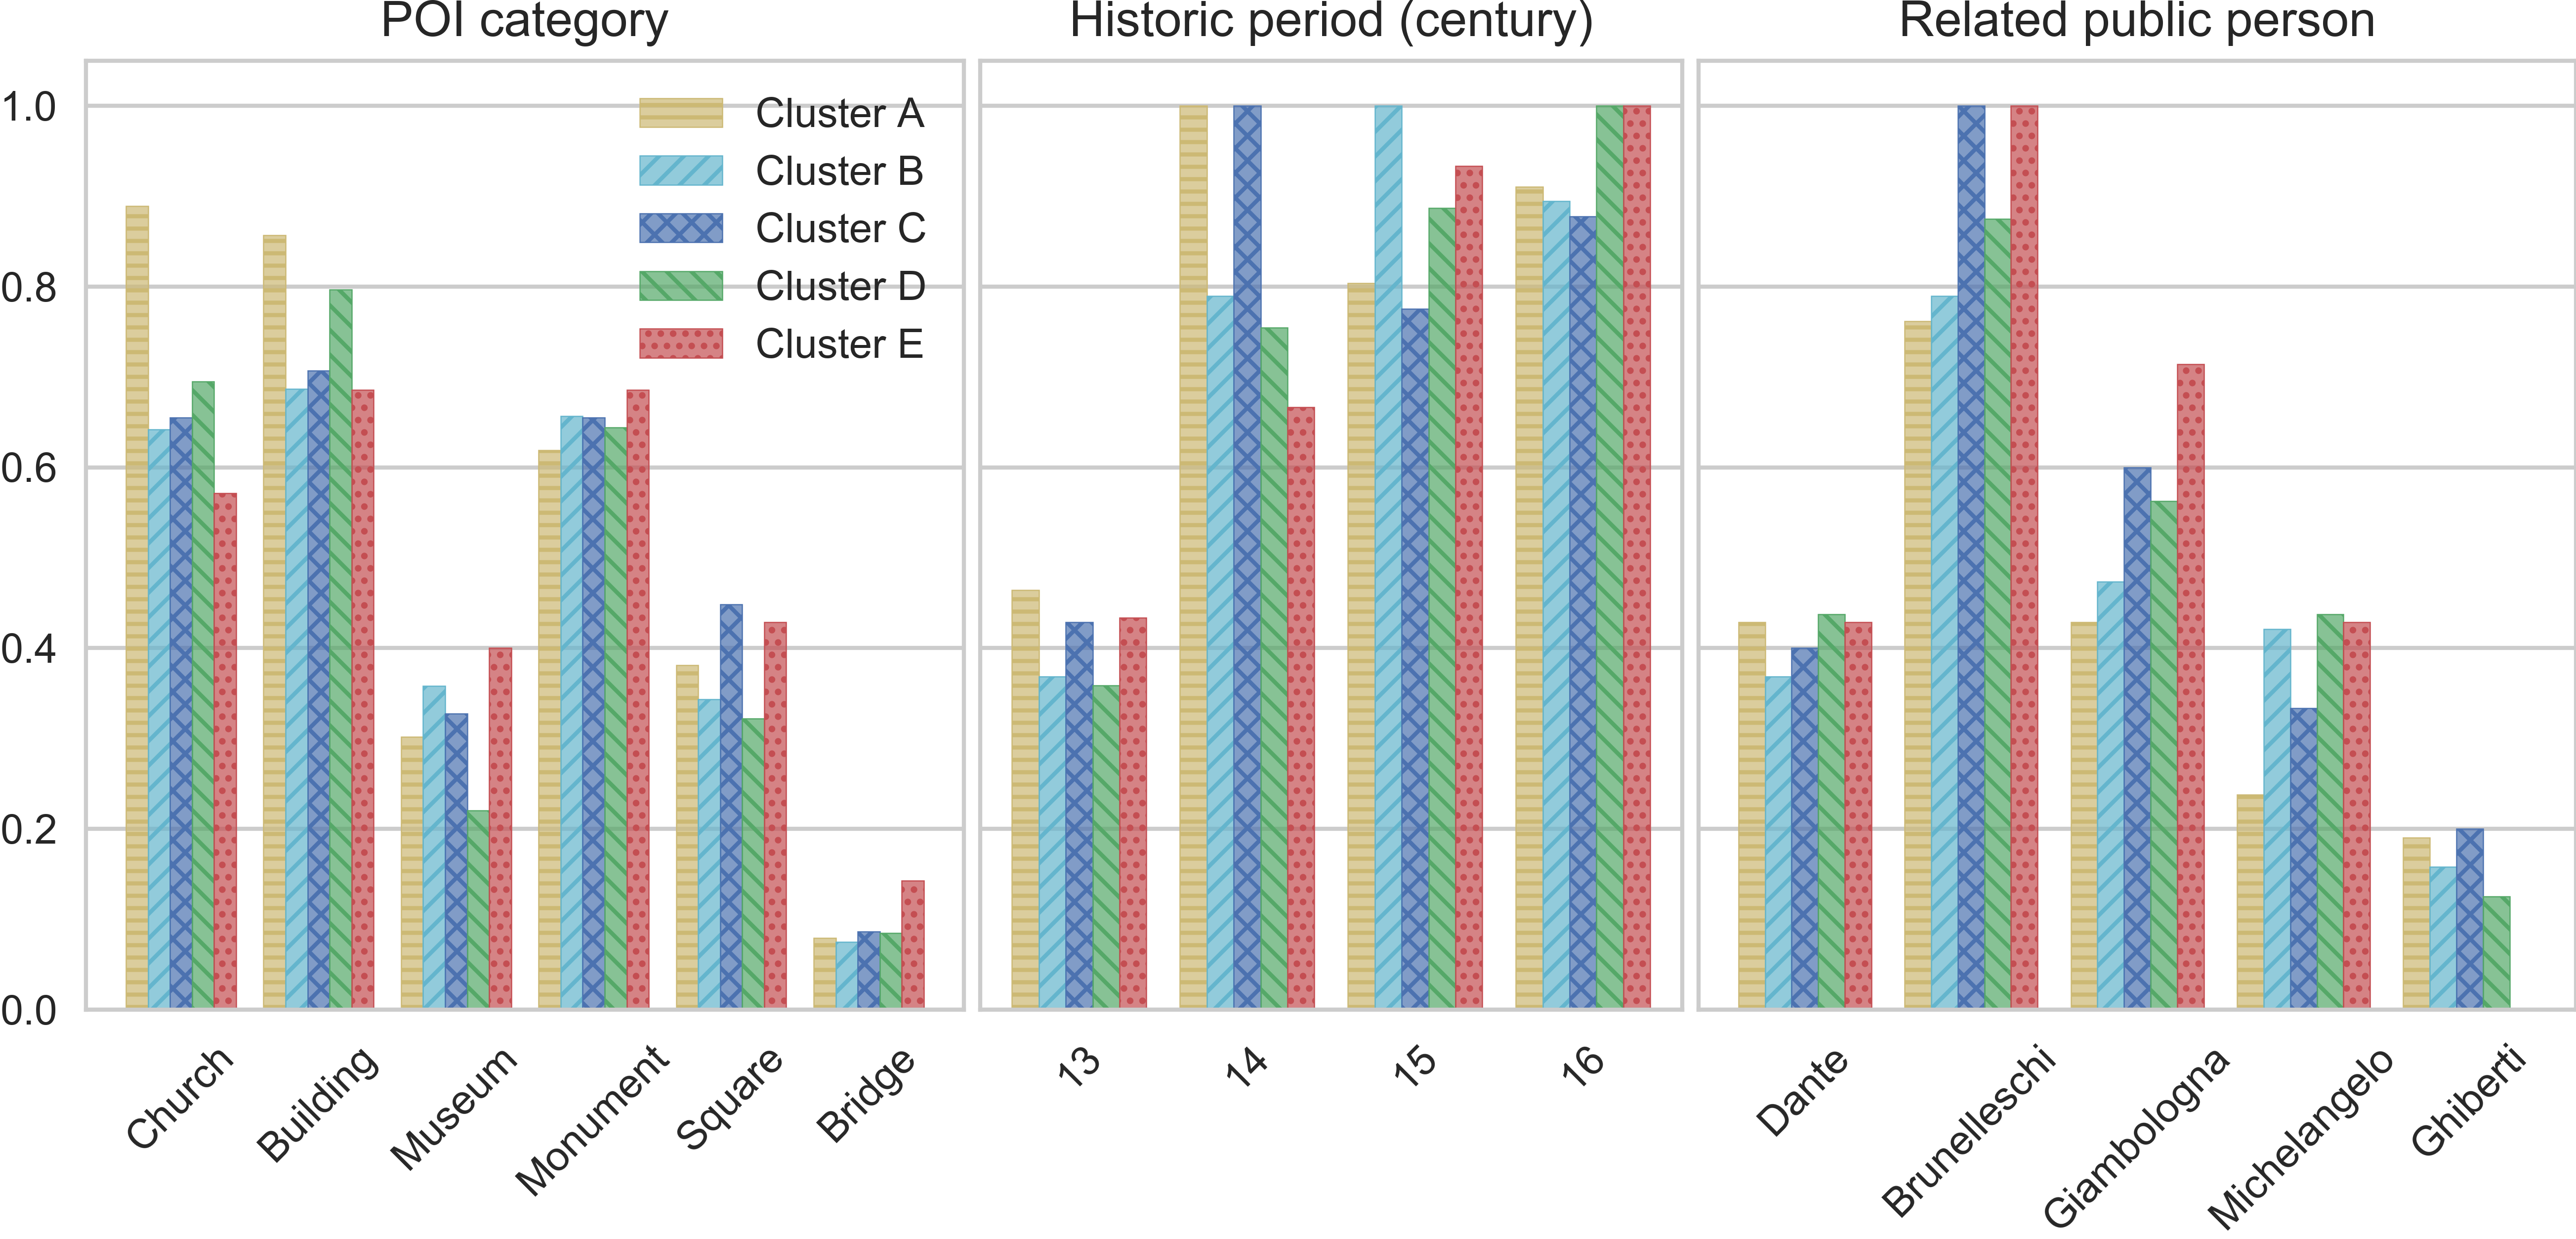
\includegraphics[width=1\linewidth]{cluster_comparison_poifeatures}
	\caption{Extract of POI features distribution per cluster.}
	\label{fig:cluster_poi}
\end{figure} 

Overall, we can see that the features variability in the clusters is not high. In fact, POIs are rather similar, i.e., they are mostly cultural POIs. It is reasonable to conjecture that if a more diverse assortment of POIs (e.g., leisure, restaurant, bar, etc.) were available then the clusters may have better discriminated alternative groups/types of tourists. Nevertheless, by looking at the specific POI descriptive features, one can notice interesting differences. For instance, POI categories like churches and buildings characterise mostly visits in clusters A and D, whereas to a lower extent trajectories in the other clusters (e.g., cluster E). Instead, cluster E is more representative of visits to bridges, squares and museums. Also POI historic period and POI related person features differentiate the clusters. For instance, cluster E is characterised by visits to POIs from the $15^{th}$ and $16^{th}$ centuries and artists from these times (i.e., Brunelleschi, Michelangelo and Giambologna).
Other relations between historic period and related person can be identified in $13^{th}$ century and Dante (e.g., clusters A and C) as well as $13^{th}$ century and Ghiberti (e.g., cluster A). Carrying out this analysis with a domain expert, an art historian, could reveal more similarities and differences between the clusters. 

In Figure \ref{fig:cluster_contex} we show the probabilities to observe certain context features in the clusters. For instance, by looking at the clusters C and E we can see that they mainly group  visits during cloudy days (left). Considering instead the temperature (centre), the clusters capture other nuances of the visits. For instance, cluster A represents visits in cold days, whereas cluster C groups visits in warmer days. Interestingly, focusing on the part of the day (right), there are clusters that represent visits performed at different times. For instance, mornings and afternoons in cluster A, afternoons and evenings in clusters B and over the whole day cluster D. 

By means of a $\chi^2$ test of independence, it has been found that the frequency of POI category, historic period, related person and weather depend on the cluster (all significant with $p<0.04$).

\begin{figure}
	\centering
	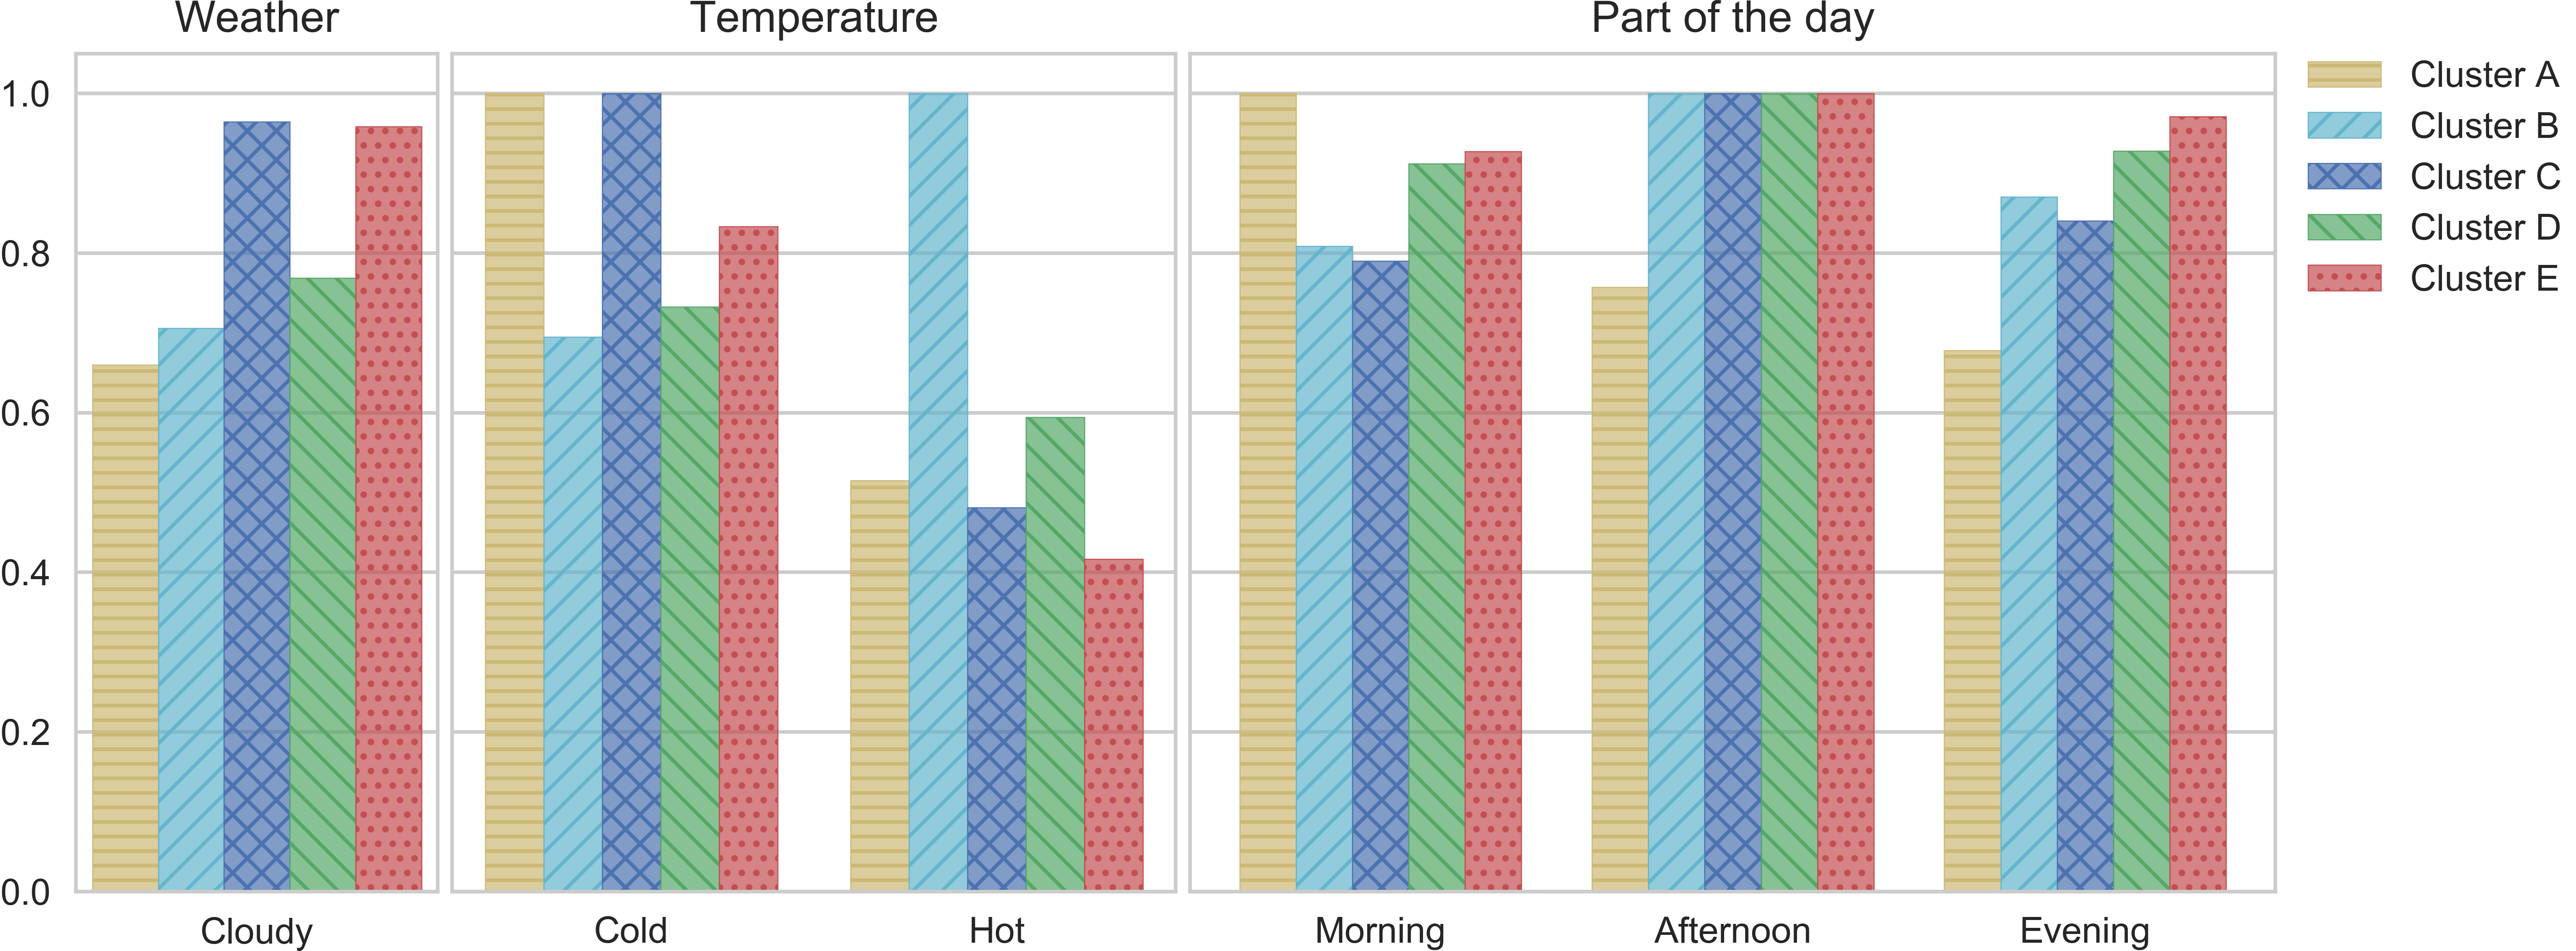
\includegraphics[width=1\linewidth]{cluster_comparison_contextfeatures}
	\caption{Extract of context features distribution per cluster.}
	\label{fig:cluster_contex}
\end{figure}

\subsection{MDP modelling}
%FR questa parte messa qui separata dal 4.3.1 non ha molto senso. Avrebbe piu' senso dire in 4.3.1 qualcosa di piu' sulla rappresentazione dello stato nelle nostre applicazioni e magari qui dare solo i dettagli. Ma forse questi dettagli si possono dare quando parli del data set delle traiettorie. Puoi descrivere il tuo MDP prima di parlare di clustering. 

We model each POI-visit trajectory in a cluster as the itinerary followed by a user, who is belonging to a group of like-minded users, that is taking decision as to optimize an (unknown) reward function common to all the users in the cluster. This problem is modelled as an MDP. 
%%FR sono un po' confuso. Il modello MDP lo hai mostrato nella sezione 4.3.1 Qui devi fare riferimento al modello generale e dire come i vari ingredienti si concretizzano per questa applicazione al turismo che usa questo particolare data set.

Let $P$ be the set of POIs visited by the users and let $\phi(s)$ 
%%FR e' la stessa phi di cui parlavi prima? Metti delle connessioni. phi e' la rappresentazione dello stato. E' lo stato un poi? Sembra che usi i due termini in maniera intercambiabile, ma devi fare distinzione tra i due, perche' non sono la stessa cosa. Il POI e' il punto di interesse, lo stato rappresenta la presenza del turista nel punto di interesse in un particolare contesto.
be the binary vector that represents for each POI the presence or absence of the following attributes: weather \textit{$f_w$}, where $w \in$ \textit{$\{$clear, foggy, partly cloudy, mostly cloudy, rainy, windy$\}$}; temperature \textit{$f_t$}, where $t \in $ \textit{$\{$freezing, cold, warm,hot$\}$}; daytime \textit{$f_d$}, where $d \in$ \textit{$\{$morning, afternoon, evening, night$\}$}; 
POI category \textit{$f_c$}, where $c \in$ \textit{$\{$church, \dots, palace$\}$}; historic period \textit{$f_h$}, where $h \in$  \textit{$\{3^{rd}$ century, \dots, $20^{th}$ century$\}$}; related person \textit{$f_r$}, where $r \in$ \textit{$\{$Brunellschi, \dots, Vasari$\}$}. 
In total there are 151 Boolean features ($F=151$), 137 representing the POI ($X=137$) and 14 representing the context ($C=14$). 

We define the state space as $S = P \times C $ where a state $s$ models the visit of a tourist at a specific POI in context.

In our problem a tourist can reach from a POI any other POI, therefore the set of actions is $A=P$. It is important to highlight that reaching a POI to visit next, i.e., performing an action, is a stochastic process: following action $a$ to reach a next POI may lead to the desired place with different context conditions, e.g., at Battistero can be rainy or foggy.

We denote with $\zeta_u$ a user $u$ trajectory, which is a temporally ordered list of states. For instance, $\zeta_{u_1} = (s_{10}, s_5, s_{15})$ represent a user $u_1$ trajectory starting from state $s_{10}$, moving to $s_5$ and ending to $s_{15}$.
%%FR queste cose le hai gia' dette.

The transition model $T$ is derived from the clustered trajectories.
%%FR queste cose le hai gia' dette.
Since we are interested in learning long term reward, i.e., optimizing for the whole visit, we set $\gamma=0.9$.


\subsection{Tourist behaviour}
In the second version of the thesis I will show the learnt behaviour models (per cluster) by showing why user's acted in a specific way. 
%%FR non e' molto chiaro cosa vuoi mostrare.
%!TEX root = ../thesis.tex
%*******************************************************************************
%****************************** Third Chapter **********************************
%*******************************************************************************
\chapter{Harnessing user behaviour models for next-item recommendation}
\label{cha:recommendation}
% **************************** Define Graphics Path **************************
\ifpdf
    \graphicspath{{Chapter5/Figs/Raster/}{Chapter5/Figs/PDF/}{Chapter5/Figs/}}
\else
    \graphicspath{{Chapter5/Figs/Vector/}{Chapter5/Figs/}}
\fi

\section{Recommendation strategies}
\begin{itemize}
\item IRL-based
\begin{itemize}
	\item Q-BASE
	\item Q-PREFERENCE
	\item Q-POP
	\item Q-POP PUSH
\end{itemize}
\item Content-based
\end{itemize}

\section{Case study: off-line performance of next-POI recommendations}
\dots and some more 

\section{Case study: User evaluation of next-POI recommendations}
\dots and some more 


%!TEX root = ../thesis.tex
%*******************************************************************************
%****************************** Third Chapter **********************************
%*******************************************************************************
\chapter{Transferring the behaviour learnt in an area (city) to other areas (city)}

% **************************** Define Graphics Path **************************
\ifpdf
    \graphicspath{{Chapter6/Figs/Raster/}{Chapter6/Figs/PDF/}{Chapter6/Figs/}}
\else
    \graphicspath{{Chapter6/Figs/Vector/}{Chapter6/Figs/}}
\fi

\section{Problem statement}


%!TEX root = ../thesis.tex
%*******************************************************************************
%****************************** Third Chapter **********************************
%*******************************************************************************
\chapter{Exploiting off-line and on-line user behaviour for next-POI recommendations in a real application: the case of Wondervalley}
\label{cha:wondervalley}
% **************************** Define Graphics Path **************************
\ifpdf
    \graphicspath{{Chapter7/Figs/Raster/}{Chapter7/Figs/PDF/}{Chapter7/Figs/}}
\else
    \graphicspath{{Chapter7/Figs/Vector/}{Chapter7/Figs/}}
\fi


%!TEX root = ../thesis.tex
%*******************************************************************************
%****************************** Third Chapter **********************************
%*******************************************************************************
\chapter{Discussion and Conclusion}

% **************************** Define Graphics Path **************************
\ifpdf
    \graphicspath{{Chapter7/Figs/Raster/}{Chapter7/Figs/PDF/}{Chapter7/Figs/}}
\else
    \graphicspath{{Chapter7/Figs/Vector/}{Chapter7/Figs/}}
\fi




% ********************************** Back Matter *******************************
% Backmatter should be commented out, if you are using appendices after References
%\backmatter

% ********************************** Bibliography ******************************
\begin{spacing}{0.9}

% To use the conventional natbib style referencing
% Bibliography style previews: http://nodonn.tipido.net/bibstyle.php
% Reference styles: http://sites.stat.psu.edu/~surajit/present/bib.htm

\bibliographystyle{apalike}
%\bibliographystyle{unsrt} % Use for unsorted references  
%\bibliographystyle{plainnat} % use this to have URLs listed in References
\cleardoublepage
\bibliography{References/references} % Path to your References.bib file


% If you would like to use BibLaTeX for your references, pass `custombib' as
% an option in the document class. The location of 'reference.bib' should be
% specified in the preamble.tex file in the custombib section.
% Comment out the lines related to natbib above and uncomment the following line.

%\printbibliography[heading=bibintoc, title={References}]


\end{spacing}

% ********************************** Appendices ********************************

\begin{appendices} % Using appendices environment for more functunality

%%!TEX root = ../thesis.tex
% ******************************* Thesis Appendix A ****************************
\chapter{How to install \LaTeX} 

\section*{Windows OS}

\subsection*{TeXLive package - full version}
\begin{enumerate}
\item	Download the TeXLive ISO (2.2GB) from\\
\href{https://www.tug.org/texlive/}{https://www.tug.org/texlive/}
\item	Download WinCDEmu (if you don't have a virtual drive) from \\
\href{http://wincdemu.sysprogs.org/download/}
{http://wincdemu.sysprogs.org/download/}
\item	To install Windows CD Emulator follow the instructions at\\
\href{http://wincdemu.sysprogs.org/tutorials/install/}
{http://wincdemu.sysprogs.org/tutorials/install/}
\item	Right click the iso and mount it using the WinCDEmu as shown in \\
\href{http://wincdemu.sysprogs.org/tutorials/mount/}{
http://wincdemu.sysprogs.org/tutorials/mount/}
\item	Open your virtual drive and run setup.pl
\end{enumerate}

or

\subsection*{Basic MikTeX - \TeX~ distribution}
\begin{enumerate}
\item	Download Basic-MiK\TeX (32bit or 64bit) from\\
\href{http://miktex.org/download}{http://miktex.org/download}
\item	Run the installer 
\item	To add a new package go to Start >> All Programs >> MikTex >> Maintenance (Admin) and choose Package Manager
\item	Select or search for packages to install
\end{enumerate}

\subsection*{TexStudio - \TeX~ editor}
\begin{enumerate}
\item	Download TexStudio from\\
\href{http://texstudio.sourceforge.net/\#downloads}
{http://texstudio.sourceforge.net/\#downloads} 
\item	Run the installer
\end{enumerate}

\section*{Mac OS X}
\subsection*{MacTeX - \TeX~ distribution}
\begin{enumerate}
\item	Download the file from\\
\href{https://www.tug.org/mactex/}{https://www.tug.org/mactex/}
\item	Extract and double click to run the installer. It does the entire configuration, sit back and relax.
\end{enumerate}

\subsection*{TexStudio - \TeX~ editor}
\begin{enumerate}
\item	Download TexStudio from\\
\href{http://texstudio.sourceforge.net/\#downloads}
{http://texstudio.sourceforge.net/\#downloads} 
\item	Extract and Start
\end{enumerate}


\section*{Unix/Linux}
\subsection*{TeXLive - \TeX~ distribution}
\subsubsection*{Getting the distribution:}
\begin{enumerate}
\item	TexLive can be downloaded from\\
\href{http://www.tug.org/texlive/acquire-netinstall.html}
{http://www.tug.org/texlive/acquire-netinstall.html}.
\item	TexLive is provided by most operating system you can use (rpm,apt-get or yum) to get TexLive distributions
\end{enumerate}

\subsubsection*{Installation}
\begin{enumerate}
\item	Mount the ISO file in the mnt directory
\begin{verbatim}
mount -t iso9660 -o ro,loop,noauto /your/texlive####.iso /mnt
\end{verbatim}

\item	Install wget on your OS (use rpm, apt-get or yum install)
\item	Run the installer script install-tl.
\begin{verbatim}
	cd /your/download/directory
	./install-tl
\end{verbatim}
\item	Enter command `i' for installation

\item	Post-Installation configuration:\\
\href{http://www.tug.org/texlive/doc/texlive-en/texlive-en.html\#x1-320003.4.1}
{http://www.tug.org/texlive/doc/texlive-en/texlive-en.html\#x1-320003.4.1} 
\item	Set the path for the directory of TexLive binaries in your .bashrc file
\end{enumerate}

\subsubsection*{For 32bit OS}
For Bourne-compatible shells such as bash, and using Intel x86 GNU/Linux and a default directory setup as an example, the file to edit might be \begin{verbatim}
edit $~/.bashrc file and add following lines
PATH=/usr/local/texlive/2011/bin/i386-linux:$PATH; 
export PATH 
MANPATH=/usr/local/texlive/2011/texmf/doc/man:$MANPATH;
export MANPATH 
INFOPATH=/usr/local/texlive/2011/texmf/doc/info:$INFOPATH;
export INFOPATH
\end{verbatim}
\subsubsection*{For 64bit OS}
\begin{verbatim}
edit $~/.bashrc file and add following lines
PATH=/usr/local/texlive/2011/bin/x86_64-linux:$PATH;
export PATH 
MANPATH=/usr/local/texlive/2011/texmf/doc/man:$MANPATH;
export MANPATH 
INFOPATH=/usr/local/texlive/2011/texmf/doc/info:$INFOPATH;
export INFOPATH

\end{verbatim}



%\subsection{Installing directly using Linux packages} 
\subsubsection*{Fedora/RedHat/CentOS:}
\begin{verbatim} 
sudo yum install texlive 
sudo yum install psutils 
\end{verbatim}


\subsubsection*{SUSE:}
\begin{verbatim}
sudo zypper install texlive
\end{verbatim}


\subsubsection*{Debian/Ubuntu:}
\begin{verbatim} 
sudo apt-get install texlive texlive-latex-extra 
sudo apt-get install psutils
\end{verbatim}

%%!TEX root = ../thesis.tex
% ******************************* Thesis Appendix B ********************************

\chapter{Installing the CUED class file}

\LaTeX.cls files can be accessed system-wide when they are placed in the
<texmf>/tex/latex directory, where <texmf> is the root directory of the user’s \TeX installation. On systems that have a local texmf tree (<texmflocal>), which
may be named ``texmf-local'' or ``localtexmf'', it may be advisable to install packages in <texmflocal>, rather than <texmf> as the contents of the former, unlike that of the latter, are preserved after the \LaTeX system is reinstalled and/or upgraded.

It is recommended that the user create a subdirectory <texmf>/tex/latex/CUED for all CUED related \LaTeX class and package files. On some \LaTeX systems, the directory look-up tables will need to be refreshed after making additions or deletions to the system files. For \TeX Live systems this is accomplished via executing ``texhash'' as root. MIK\TeX users can run ``initexmf -u'' to accomplish the same thing.

Users not willing or able to install the files system-wide can install them in their personal directories, but will then have to provide the path (full or relative) in addition to the filename when referring to them in \LaTeX.



\end{appendices}

% *************************************** Index ********************************
\printthesisindex % If index is present

\end{document}
